\chapter{Spec-to-C Equivalence Checker}
\label{sec:spectocalgo}
This chapter presents our automatic equivalence checker \toolName{}.
Given a \SpecL{} and a C program along with the input-output specification for each function-pair,
\toolName{} searches for a proof of equivalence between the CFGs of each \SpecL{} and C procedures: \sprog{} and \cprog{}.
Recall that CFGs represent deterministic programs and evidently, the C procedure is determinized during conversion to \cprog{}.
Hence, \toolName{} checks equivalence between a \SpecL{} procedure and the determinized C procedure.
A translation validator (such as the Counter tool \cite{oopsla20}) can be used to check equivalence between
the same determinized C procedure against its generated assembly.
By restricting the deterministic choices made by the C compiler to the same choices made during construction of \cprog{},
we can effectively establish end-to-end equivalence between a \SpecL{} procedure against its assembly.
We start with a dataflow formulation of the points-to analysis used as part of \toolName{} on \cprog{} as well as
deconstruction programs during discharge of type III proof obligations in \cref{sec:pointsToFormal}.
As stated in \cref{sec:contribs}, \toolName{} is based on three major algortihms:
\curved{A1} an algorithm to incrementally construct a product-CFG by correlating program executions across
\sprog{} and \cprog{},
\curved{A2} an algorithm to identify inductive invariants at intermediate PCs in the (partially constructed)
product-CFG, and
\curved{A3} an algorithm for solving proof obligations generated by \curved{A1} and \curved{A2} algorithms.
We describe our counterexample-guided best-first search algorithm for construction of a product-CFG (\curved{A1}) in \cref{sec:searchalgo}.
This is followed by a dataflow formulation of our counterexample-guided invariant inference algorithm (\curved{A2}) in \cref{sec:invinferalgo}.
Recall that algorithms \curved{A1} and \curved{A2} are based on prior work on equivalence checking between unoptimized IR (aka determinized C)
and assembly \cite{shubhanipdhthesis}.
We only summarize these procedures in addition to the primary modifications made in the context of \SpecL{}-C equivalence.
The previous chapter walked through our proof discharge algorithm (\curved{A3}) using examples, ending with
the pseudocode of proof discharge algorithm (\cref{algo:proofSummary}).
In this chapter, we present pseudocode for multiple subprocedures utilized by our proof discharge algorithm in \cref{sec:proofalgo}.
Additionally, we describe the process of encoding queries in SMT logic as well as the recovery of counterexamples from models returned by SMT solvers.
We finish with a new representation of expressions, which allows us to simplify a number of steps performed
by the proof discharge algorithm.

\begin{table}
\begin{center}
\caption{\label{tab:pointstoalgodfa}Dataflow Formulation of the Points-to Analysis}
\vspace{10px}
% \begin{footnotesize}
\begin{tabular}{|l|l|}
\hline
\Tstrut \Bstrut Domain &
\begin{tabular}{@{}l@{\hskip 12mm}l@{}}
$\Delta^{\cprog{}} : (\pseudoregs{}^{\cprog{}} \cup \memregions{}) \rightarrow 2^{\memregions{}}$ &
$\Delta^{\dprog{}} : (\pseudoregs{}^{\cprog{}} \cup \memregions{} \cup \pseudoregs{}^{\dprog{}}) \rightarrow 2^{\memregions{}}$ \\
\end{tabular} \\
\hline
\Tstrut \Bstrut Direction & Forward \\
\hline
Boundary Condition &
\begin{tabular}{@{}l@{\hskip 11mm}l@{}}
\multicolumn{2}{@{}l}{\Tstrut \Bstrut $\Delta_n$ for start node :}\\
$\Delta_n^{\cprog{}}(t) = \begin{dcases} \emptyset \ \ \  t \in \pseudoregs{}^{\cprog{}} \\ \memregions{} \ \ t \in \memregions{} \end{dcases}$ &
$\Delta_n^{\dprog{}}(t) = \begin{dcases} \Delta_{n_C}^{\cprog{}}(t) \ \  t \in (\pseudoregs{}^{\cprog{}} \cup \memregions{}) \\ \emptyset \ \ \ \ \ \ \ \ \ \  t \in \pseudoregs{}^{\dprog{}} \end{dcases}$ \\
\end{tabular} \\
\hline
\Tstrut \Bstrut Initialization to $\top$ & $\Delta_n$ for non-start nodes : $\Delta_n(t) = \emptyset \ \  t \in {\tt Domain}(\Delta_n)$ \\
\hline
\makecell[l]{\Tstrut Transfer function across \\
\Bstrut edge $e = (s \rightarrow d)$} &
$\Delta_d = f_e(\Delta_s)$ (described in \cref{sec:pointsToFormal}) \\
\hline
Meet operator $\otimes$ &
\makecell[l]{\Tstrut $\Delta_n \leftarrow \Delta^1_n \otimes \Delta^2_n$ \\
\Tstrut \Bstrut $\Delta_n(t) = \Delta^1_n(t) \cup \Delta^2_n(t) \ \  t \in {\tt Domain}(\Delta_n)$} \\
\hline
\end{tabular}
% \end{footnotesize}
\end{center}
\end{table}

\section{Points-to Analysis}
\label{sec:pointsToFormal}
Recall that in \cref{sec:reconsbisim}, we needed to reason about aliasing to successfully discharge a type III proof obligation.
These aliasing relationships are introduced in \cref{sec:pointsTo} and subsequently used in \cref{sec:pointsToAsInvariants} to
successfully discharge a type III proof obligation.
An interprocedural, flow-sensitive, untyped points-to analysis is used to identify these relationships
in \cprog{} as well as each deconstruction program \dprog{}.
\Cref{tab:pointstoalgodfa} presents the dataflow formulation of our points-to analysis.
We start by identifying the set \memregions{} of all region labels representing mutually non-overlapping
regions of the \cprog{} memory \mem{}.
For each call to {\tt malloc()} at PC $A$ of \cprog{}'s IR, we add $A_1$ and $A_{2+}$ to \memregions{}.
Recall that $A_1$ represents the region of memory returned by the {\em most recent} execution of $A$.
$A_{2+}$ represents the region of memory returned by older (i.e. all but most recent) executions of $A$.
$\memregions{} = \bigcup_{A} \{ A_1, A_{2+} \} \cup \{ \heapr{} \}$,
where \heapr{} is the region of memory \mem{} not covered by the labels associated with allocation sites.
% Note that \memregions{} is computed once interprocedurally and contains
% memory regions (associated with {\tt malloc()} calls) for all procedures in the IR of $C$.

Let $\pseudoregs{}^{C}$  be the set of all scalar pseudo-registers in \cprog{}'s IR.
We use a forward dataflow analysis to identify a may-point-to function
$\Delta^{C}: (\pseudoregs{}^{C} \cup \memregions{}) \mapsto 2^{\memregions{}}$ at each program point in \cprog{}'s IR.
For a deconstruction program \dprog{}, we are also interested in finding the may-point-to function for
all scalar pseudo-registers in \dprog{}'s IR, say $\pseudoregs{}^{D}$.
Thus, the domain of the may-point-to function for \dprog{} ($\Delta^{D}$) contains $\pseudoregs{}^{D}$
in addition to the domain of $\Delta^{C}$ i.e.
$\Delta^{D}: (\pseudoregs{}^{C} \cup \memregions{} \cup \pseudoregs{}^{D}) \mapsto 2^{\memregions{}}$.
The '$\pointsTo$' operator introduced in \cref{sec:pointsTo} is called the {\em element-wise} may-point-to function
and is related to the may-point-to function $\Delta$ as follows: $p \pointsTo{} S \Leftrightarrow \Delta(p) \subseteq S$.

The meet operator is element-wise set-union e.g., $p \pointsTo{} S_1$ and $p \pointsTo{} S_2$
combines into $p \pointsTo{} S_1 \cup S_2$.
Evidently, the $\top$ value is the constant function that returns $\emptyset$.
At entry of \cprog{}, we conservatively assume that all memory regions may point to each other.
However, at entry of a deconstruction program \dprog{}, created during a proof obligation at product-CFG node $(n_S\!:\!n_C)$,
we use \cprog{}'s precomputed may-point-to function at $n_C$ ($\Delta^{C}_{n_C}$)
to initialize the points-to relationships for all state elements in \cprog{}'s IR (i.e. $\pseudoregs{}^{C} \cup \memregions{}$).
This is a crucial step for proving equality of \cprog{} values under different memory states as seen in \cref{sec:pointsToAsInvariants}.

Next, we discuss the transfer function $f_e$ for our points-to analysis.
For an IR instruction ${\tt x} \coloneqq {\tt c}$, for constant {\tt c}, the
transfer function updates $\Delta({\tt x}) \coloneqq \emptyset$.
For instruction ${\tt x} \coloneqq {\tt y\ op\ z}$ (for some arithmetic or logical operator {\tt op}),
we update $\Delta({\tt x}) \coloneqq \Delta({\tt y}) \cup \Delta({\tt z})$.
For a load instruction ${\tt x} \coloneqq \memRead{\mem{}}{y}{T}$, we
update $\Delta({\tt x}) \coloneqq \bigcup_{t \in \Delta(y)} \Delta(t)$.
For a store instruction $\mem{} \coloneqq \memWrite{\mem{}}{x}{y}{T}$, for all
$t \in \Delta({\tt x})$, we update $\Delta(t) \coloneqq \Delta(t) \cup \Delta(y)$.
For a malloc instruction ${\tt x} \coloneqq {\tt malloc}_A()$
(where $A$ represents the allocation site), we perform the following steps (in order):
\begin{enumerate}
\item Convert all existing occurrences of $A_1$ to $A_{2+}$, i.e., for all $t \in (\pseudoregs{}^{C} \cup \memregions{})$,
if $A_1 \in \Delta(t)$, then update $\Delta(t) \coloneqq (\Delta(t) \setminus \{ A_1 \}) \cup \{ A_{2+} \}$.
\item Update $\Delta({\tt x}) \coloneqq \{ A_1 \}$.
\item Update $\Delta(A_{2+}) \coloneqq \Delta(A_{2+}) \cup \Delta(A_1)$.
\item Update $\Delta(A_1) \coloneqq \emptyset$.
\end{enumerate}

For function calls, a {\em supergraph} is created by adding control flow edges
from the call-site to the procedure head (copying actual arguments to the formal arguments) and
from the procedure exit to the program point just after the
call-site (copying returned value to the variable assigned at the callsite),
e.g., in \cref{fig:clistdeconsCFG}, the dashed edges represent supergraph edges.

The allocation-site abstraction (with a bounded-depth call stack) is
known to be effective at disambiguating memory regions belonging to
different data structures
\cite{allocationSiteAbstraction82,allocationSiteAbstraction90,allocationSiteAbstraction06}.
In our work, we also need to reason about non-aliasing
of the most-recently allocated object (through a {\tt malloc} call) and
the previously-allocated objects (as in the \type{List}
construction example). The coarse-grained $\{1, 2+\}$
categorization of allocation recency is effective for such disambiguation.

\begin{figure}[t!]
\begin{tabular}{@{}c@{}c@{}c@{}}
\begin{subfigure}[b]{0.30\textwidth}
\begin{center}
{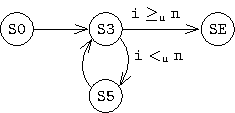
\includegraphics[scale=1.15]{chapters/figures/figMallocSpecCfg.pdf}}
\end{center}
\vspace{17px}
\caption{\label{figrr:llAllocSpecIRCFG}CFG of \SpecL{} procedure}
\end{subfigure}%
&
\begin{subfigure}[b]{0.30\textwidth}
\begin{center}
{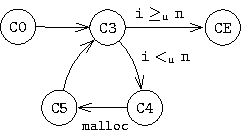
\includegraphics[scale=1.1]{chapters/figures/figMallocCCfg.pdf}}
\end{center}
\vspace{5px}
\caption{\label{figrr:llAllocCCFG}CFG of C procedure}
\end{subfigure}%
&
\begin{subfigure}[b]{0.40\textwidth}
\begin{center}
{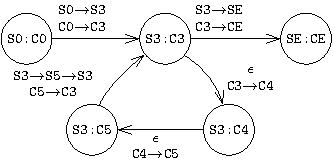
\includegraphics[scale=1.1]{chapters/figures/figMallocProductCfg.pdf}}
\end{center}
\caption{\label{figrr:llAllocProductCFG}Product-CFG}
\end{subfigure}%
\\
\end{tabular}
\caption{\label{figrr:llAllocAllCFGs}\Cref{figrr:llAllocSpecIRCFG,figrr:llAllocCCFG} shows the CFG representation of \SpecL{} and C IRs in \cref{figr:llAllocSpecIR,figr:llAllocCIR}
for the {\tt mk\_list} procedures in \cref{fig:llAllocSpec,fig:llAllocC}.
The product-CFG representing path correlations between \cref{figrr:llAllocSpecIRCFG,figrr:llAllocCCFG} is shown in \cref{figrr:llAllocProductCFG}.}
\end{figure}
\begin{figure}
\begin{algorithm}[H]
\begin{footnotesize}
\SetAlgoLined
\SetKwProg{Fn}{Function}{}{end}
\Fn{$bestFirstSearch(\sprog{},\cprog{},\mu)$}{
  $\pi_{init} \mapsfrom createInitProductCFG(\sprog{},\cprog{})$;\\
  $Q \mapsfrom \{ \pi_{init} \}$;\\
  \While{$Q \keyword{is\ not} empty$}{
    $\pi_{cur} \mapsfrom extractMostPromising(Q)$;\\
    ${\tt InferInvariantsAndCounterexamples}(\pi_{cur})$;\\
    \
    \uIf{$getPathsetToCorrelate(\cprog{},\pi_{cur}) = \cons{Found}(\xi_C)$}{
      \ForEach{$\xi_S \keyword{in} enumeratePathsetsInS(\sprog{},\xi_C,\mu)$}{
        $\pi_{next} \mapsfrom extendProductCFG(\pi_{cur},\xi_S,\xi_C)$;\\
        $Q \mapsfrom Q \cup \{ \pi_{next} \}$;\\
      }
    }
    \ElseIf{$productCFGRepresentsBisim(\pi_{cur})$}{
      \Return{$\cons{Found}(\pi_{cur})$};\\
    }
  }
  \Return{$\cons{NotFound}$};\\
}
\end{footnotesize}
\caption{\label{algo:search}Pseudocode for Best-First-Search Procedure for construction of Product-CFG}
\end{algorithm}
\end{figure}

\section{Counterexample-guided Product-CFG Construction}
\label{sec:searchalgo}
\toolName{} constructs a product-CFG incrementally to search for a bisimulation relation
between the \SpecL{} and C CFGs : \sprog{} and \cprog{}.
Multiple candidate product-CFGs are partially constructed during this search;
the search completes when one of these candidates yield an equivalence proof.
Recall that the incremental product-CFG construction algorithm is based on prior work \cite{shubhanipdhthesis}
and we simply summarize the relevant components in the context of \SpecL{}-C equivalence.

{\em Anchor nodes} are identified in \sprog{} and \cprog{}, and represents the
CFG nodes (i.e. IR PCs) being considered for correlation.
The algorithm ensures that every cycle in both \sprog{} and \cprog{} contains at least one anchor node.
The start and exit nodes are always anchor nodes.
Also, for every function call, the nodes just before and after its callsite are considered anchor nodes.
For example, in \cref{figrr:llAllocCCFG}, \cpc{4} and \cpc{5} are anchor nodes around the call to {\tt malloc}.
A valid selection of anchor nodes for the CFGs in \cref{figrr:llAllocSpecIRCFG,figrr:llAllocCCFG} are:
$\{ \spc{0},\spc{3},\spc{E} \}$ and $\{ \cpc{0}, \cpc{3}, \cpc{4}, \cpc{5}, \cpc{E} \}$ respectively.
For each anchor node in \cprog{}, our search algorithm searches for a correlated anchor node in \sprog{} --- if
a (partially constructed) product-CFG $\pi$ contains a product-CFG node  $(n_S\!:\!n_C)$, then $\pi$
correlates node $n_C$ in \cprog{} with node $n_S$ in \sprog{}.
The search procedure begins with a single partially-constructed product-CFG $\pi_{init}$.
$\pi_{init}$ contains exactly one node (\scpc{0}{0}) that encodes the correlation of the entry nodes
(i.e. \spc{0} and \cpc{0}) of \sprog{} and \cprog{}.

\subsection{Correlating Pathsets}
\label{sec:pathsetcorrel}
Recall that a product-CFG edge correlates transitions in \sprog{} and \cprog{}.
The examples presented so far only considers correlations between {\em paths} in \sprog{} and \cprog{}.
However, we consider a more general approach of {\em pathset} correlations in the context of product-CFG construction.
Pathsets are based on earlier work on the Counter tool \cite{oopsla20,shubhanipdhthesis}
and help improve the completeness of the bisimulation search by considering correlations of a single path in \cprog{}
with a set of paths in \sprog{} and vice versa, where individual paths may be uncorrelated.
An example of such a scenario is depicted in \cref{sec:strchrexample}.
For now, we briefly summarize pathsets in the context of \SpecL{}-C bisimulation search.
A {\em pathset} $\xi$ is essentially a set of paths with the following additional properties:
(a) all paths $\rho \in \xi$ begin at the same node and terminate at the same node, and
(b) all paths $\rho \in \xi$ are mutually exclusive i.e. {\em at most} one of ${\tt pathcond}_{\rho}$ can be true.
A $(\mu,\delta)$-{\em unrolled pathset} $\xi$ is a pathset from $n_s$ to $n_d$ such that:
(a) all paths $\rho \in \xi$ contains {\em at most} $\mu$ occurrences of {\em any} node except $n_d$ as the end node (to-PC) of an edge in $\rho$, and
(b) all paths $\rho \in \xi$ contains {\em exactly} $\delta$ occurrences of $n_d$ as the end (to-PC) of an edge in $\rho$.
Intuitively, $\delta$ represents the number of iterations of a loop (ending at $n_d$) considered as part of a path in $\xi$,
whereas $\mu$ bounds the number of times any node is visited by a path in $\xi$.
$(\mu,\delta)$-unrolled pathsets have been shown to be quite effective at identifying correlations in the presence of
compiler transformations such as unrolling and vectorization \cite{shubhanipdhthesis} and we also found it to be
suitable in the context of \SpecL{}-C equivalence.

At each step of the incremental construction process, a node $(n_S \! : \! n_C)$ is chosen in a product-CFG $\pi$
and a (1,1)-unrolled pathset $\xi_C$ in \cprog{} starting at $n_C$ (and ending at an anchor node) is selected ({\tt getPathsetToCorrelateInC()}).
Then, we enumerate $(\mu_S,\delta)$-unrolled pathsets in \sprog{} (for $\delta \in [0,\mu_S]$) as potential correlations for
the pathset $\xi_C$ in \cprog{} ({\tt enumeratePathsetsInS()}).
$\mu_S$ is a fixed parameter of \toolName{} and is called the {\em unroll factor}.
For example, during construction of the product-CFG shown in \cref{figrr:llAllocProductCFG},
say we select the product-CFG node (\scpc{3}{3}).
We choose the \cprog{} path(set) \cpath{3,4} and enumerate its potential correlations (i.e. $(\mu_S,\delta)$-unrolled pathsets in \sprog{} starting at \spc{3}):
$\epsilon$, \spath{3,5,3}, \ldots, $\pathset{S3,(\pathset{S5,S3})^{\mu_S}}$.
Importantly, for pathsets $\xi_S$ (in \sprog{}) and $\xi_C$ (in \cprog{}) to be considered for correlation,
they must originate and terminate at anchor nodes, i.e. the path \spath{3,5} is skipped during enumeration.
Moreover, the pathset $\xi_C$ may only contain anchor nodes as its source and destination.
Thus, the path \cpath{3,4,5} is not considered for $\xi_C$,
instead we attempt to correlate the subpaths \cpath{3,4} and \cpath{4,5} individually.
\Cref{sec:pathsethoaretriples} briefly discusses the techniques of handling Hoare triples (i.e. proof obligations)
involving pathsets.

For each enumerated correlation possibility $(\xi_S,\xi_C)$, a separate product-CFG $\pi'$ is
created (by cloning $\pi$) and a new product-CFG edge $e=(\xi_S,\xi_C)$ is added to $\pi'$ ({\tt extendProductCFG()}).
The head of the product-CFG edge $e$ is the (potentially newly added) product-CFG node representing
the correlation of the end-points of pathsets $\xi_S$ and $\xi_C$. For example, the node (\scpc{3}{4}) is added
to the product-CFG if it correlates pathsets $\epsilon$ and \cpath{3,4} starting at (\scpc{3}{3}).
Recall that, we consider $\epsilon$ as a candidate for $\xi_S$, but not $\xi_C$.
The algorithm ensures that no cycle in \cprog{} is correlated with $\epsilon$ in \sprog{}
(to preserve divergence discussed in \cref{sec:bisim}).
For each node $n$ in a product-CFG $\pi$, we maintain a small number of
concrete machine state pairs (of \sprog{} and \cprog{}).
The concrete machine state pairs at $s$ are obtained as counterexamples to unsucessful proof
obligations \hoareTriple{\phi_s}{s \rightarrow d}{\phi_d} (for some edge $s \rightarrow d$ and node $d$ in $\pi$).
Thus, by construction, these counterexamples represent concrete state pairs that may potentially occur
at $n$ during the lockstep execution encoded by $\pi$.

\subsection{Best-First Ranking of Partial Product-CFGs}
\label{sec:rankproductcfg}
To evaluate the promise of a possible correlation $(\xi_S,\xi_C)$ starting at node $n$
in product-CFG $\pi$, we examine the execution behaviour of the counterexamples at $n$ on
the product-CFG edge $e=(s\rightarrow d)=(\xi_S,\xi_C)$.
If the counterexamples ensure that the machine states remain related at $d$,
then that candidate correlation is ranked higher.
This ranking criterion is based on prior work \cite{oopsla20}.
A best-first search (BFS) procedure based on this ranking criterion is used to incrementally construct
a product-CFG (starting from $\pi_{init}$).
For each intermediate candidate product-CFG $\pi$ generated during this search procedure,
an automatic invariant inference procedure (discussed next in \cref{sec:invinferalgo}) is
used to identify invariants at all the nodes in $\pi$ ({\tt InferInvariantsAndCounterexamples()}).
The counterexamples obtained from the proof obligations generated by this invariant inference
procedure are added to the respective nodes in $\pi$; these counterexamples help rank
future correlations starting at those nodes.

If after invariant inference, we realize that an intermediate candidate product-CFG $\pi_1$
is not promising enough, we backtrack and choose another candidate product-CFG $\pi_2$
and explore the potential correlations that can be added to $\pi_2$ ({\tt extractMostPromising()}).
Thus, a product-CFG is constructed one edge at a time.
If at any stage, a product-CFG $\pi$ satisfies the well-formedness conditions (introduced in \cref{sec:wellformedproductcfg})
and invariants ensure equal observables (i.e. \post{} holds at correlated exit nodes),
we have successfully shown equivalence ({\tt productCFGRepresentsBisim()}).
This counterexample-guided BFS procedure is similar to the one described in prior work on
the Counter algorithm \cite{oopsla20}.

\subsection{Correlation in the Presence of Function Calls}
\label{sec:correlfcalls}
Recall that \sprog{} and \cprog{} may make function calls (including self calls),
e.g., C memory allocation, recursive traversal of a tree data structure.
Recall that the nodes just before and after a function call are always considered anchor nodes.
Calls to memory allocation functions in \cprog{} (i.e. {\tt malloc}) are handled by correlating
the function call edge with the empty path ($\epsilon$) in \sprog{}.
For example, in the product-CFG shown in \cref{figrr:llAllocProductCFG}, the {\tt malloc} edge \cpath{4,5} in \cprog{}
is correlated with $\epsilon$ in \sprog{}.

For all other calls, our correlation algorithm (in \cref{sec:searchalgo}) ensures that the anchor nodes
around such a callsite are correlated one-to-one across both procedures.
For example, let there be a call to procedure $\delta$ in \sprog{} at PC $n_S$, i.e. $n_S$ is the call-site.
Let us denote the program point just after this call-site as $n'_S$.
Let {\tt args}$_{n_S}$ represent the values of the actual arguments of this function call (at $n_S$).
Let {\tt ret}$_{n'_S}$ represent the value returned by this function call (at $n'_S$).
Similarly, for a procedure call $\delta$ in \cprog{}, let $n_C$, $n'_C$, {\tt args}$_{n_C}$ and {\tt ret}$_{n'_C}$
represent the function call-site, program point just after the call-site,
the values of the actual arguments and the value returned respectively.
Our algorithm ensures that the only correlation possible in a product-CFG $\pi$ for these program points are
$(n_S:n_C)$ and $(n'_S:n'_C)$.

We utilize the user-supplied input-output specification for $\delta$, say $(\pre{}_{\delta},\post{}_{\delta})$,
to obtain the desired invariants at nodes $(n_S:n_C)$ and $(n'_S:n'_C)$ in the product-CFG.
A successful proof must {\em ensure} that $Pre_{\delta}$({\tt args}$_{n_S}$,{\tt args}$_{n_C}$) holds at $(n_S:n_C)$.
Further, the proof can {\em assume} that $Post_{\delta}$({\tt ret}$_{n'_S}$,{\tt ret}$_{n'_C}$) holds at $(n'_S:n'_C)$.
Note that {\tt args}$_{n_C}$ and {\tt ret}$_{n'_C}$ includes the \cprog{} memory states
$\mem{}_{n_C}$ (at $n_C$) and $\mem{}_{n'_C}$ (at $n'_C$) respectively.
Thus, for function calls, we inductively prove the precondition (on the arguments) at $(n_S:n_C)$
and assume the postcondition (on the returned values) at $(n'_S:n'_C)$.

\begin{table}[H]
\begin{center}
\caption{\label{tab:dataflow_formulation}Dataflow formulation for the Invariant Inference Algorithm.}
\setlength{\belowcaptionskip}{-30pt}
\begin{footnotesize}
\begin{tabular}{|l|l|}
\hline
Domain &
\makecell[c]{
\ldelim\{{2}{3mm}{\footnotesize \ \  $\phi_n$ is a conjunction of predicates drawn from\ \ }\rdelim\}{2}{3mm} \\ \ {\footnotesize grammar in \ref{fig:invGrammar}, $\Gamma_n$ is a set of counterexamples}} \\
\hline
Direction & Forward\\
\hline
\makecell[l]{Transfer function across \\ edge $e=(s\rightarrow d)$} & $(\phi_d,\Gamma_d) = f_e(\phi_s,\Gamma_s)$ (\cref{algo:tf})\\
\hline
\begin{tabular}{@{}l@{}}
Meet operator $\otimes$\\
{\footnotesize $(\phi_n,\Gamma_n) \leftarrow (\phi^1_n,\Gamma^1_n) \otimes (\phi^2_n,\Gamma^2_n)$}\\
\end{tabular}
& $\Gamma_n \leftarrow \Gamma^1_n\cup \Gamma^2_n$, \ \ \ \ \ \ \ \ $\phi_n \leftarrow \mathrm{\it StrongestInvCover}(\Gamma_n)$\\
\hline
Boundary condition & {\tt out[$n^{start}$]} = {\tt $(Pre,\Gamma_{n^{start}})$}\ \ \ \ \ \\
\hline
Initialization to $\top$ & {\tt in[$n$] = $($False,$\{\})$} for all non-start nodes\\
\hline
\end{tabular}
\end{footnotesize}
\end{center}
\end{table}
\vspace{-10px}
\begin{figure}[H]
\begin{center}
\begin{subfigure}{.58\textwidth}
\begin{algorithm}[H]
\begin{footnotesize}
\SetAlgoLined
\SetKwProg{Fn}{Function}{}{end}
\Fn{$f_e(\phi_s, \Gamma_s)$}{
  $\Gamma^{can}_{d} \mapsfrom \Gamma_{d} \cup {\tt exec}_e(\Gamma_s)$;\\
  $\phi^{can}_{d} \mapsfrom \mathrm{\it StrongestInvCover}(\Gamma^{can}_{d})$;\\
  \While{{\tt SAT$(\neg(\{\phi_s\} (e) \{\phi^{can}_{d}\}), \gamma_s)$}}
  {
    $\gamma_{d} \ \ \ \ \mapsfrom {\tt exec}_e(\gamma_s)$;\\
    $\Gamma^{can}_{d} \mapsfrom \Gamma^{can}_{d}\cup\gamma_{d}$;\\
    $\phi^{can}_{d} \mapsfrom \mathrm{\it StrongestInvCover}(\Gamma^{can}_{d})$;\\
  }
  \Return{$(\phi^{can}_{d}, \Gamma^{can}_{d})$;}\\
}
\end{footnotesize}
\end{algorithm}
\caption{\label{algo:tf} Transfer function $f_e$ across
edge $e=(s\rightarrow d)$.}
\end{subfigure}%
\hfill
\rulesep
\hfill
\begin{subfigure}{.40\textwidth}
\begin{center}
\begin{footnotesize}
\begin{tabular}{p{0.45cm}p{0.15cm}l}
${Inv}$ & $\rightarrow$ & $\sum_{i}{c_i v_i}=c$ $|$ $v_1 \odot v_2$  \\
% & $|$ & $v_1 \odot v_2$ \\
& $\ \ |$ & $\alpha_S = {\tt liftC}_m(v^C \dots)$ \\
\end{tabular}
\end{footnotesize}
\end{center}
\vspace{-10px}
\caption{\label{fig:invGrammar}\footnotesize Predicate grammar for constructing invariants. $v$ represents a bitvector variable in either $S$ or $C$. $c$ represents a bitvector constant. $\odot$ $\in$ $\{<,\leq\}$. $\alpha_S$ represents an ADT variable in \SpecL{}. $v^{C}$ represents a bitvector variable in $C$. $m$ represents the current $C$ memory state.}
\end{subfigure}%
\caption{Transfer function $f_e$ and Predicate grammar $Inv$ for invariant inference dataflow analysis in \cref{tab:dataflow_formulation}.
Given invariants ($\phi_{s}$) and counterexamples ($\Gamma_{s}$) at node $s$,
$f_e$ returns the updated
invariants ($\phi_{d}$) and counterexamples ($\Gamma_{d}$) at
node $d$.
{\em StrongestInvCover($\Gamma$)} computes the strongest invariant cover for counterexamples $\Gamma$.
{\tt exec$_e$($\Gamma$)} (concretely) executes
counterexamples $\Gamma$ over edge $e$.
{\tt SAT($\phi$, $\gamma$)} determines
the satisfiability of $\phi$; if satisfiable, the models (counterexamples) are returned in output parameter $\gamma$.}
\end{center}
\end{figure}

\section{Invariant Inference and Counterexample Generation}
\label{sec:invinferalgo}
We formulate our counterexample-guided invariant inference algorithm as a forward dataflow analysis
as shown in \cref{tab:invinferalgodfa}.
The invariant inference procedure is responsible for inferring invariants $\phi_n$ at each intermediate
node $n$ of a (partially constructed) product-CFG, while also generating a set of counterexamples
$\Gamma_n$ that represents the potential concrete machine states at $n$.
Recall that the invariant inference algorithm is based on prior work \cite{shubhanipdhthesis}
and we simply summarize the relevant components in the context of \SpecL{}-C equivalence.

Given the invariants and counterexamples at node $s$: ($\phi_s,\Gamma_s$),
the transfer function initializes the new candidate set of counterexamples at $d$ ($\Gamma^{can}_{d}$)
with the current set of counterexamples at $d$ ($\Gamma_{d}$) {\em union}-ed with
the counterexamples obtained by executing $\Gamma_s$ on edge $e$ (through {\tt exec}$_e$).
The candidate invariant at $d$ ($\phi^{can}_d$) is computed as the strongest cover
of $\Gamma^{can}_{d}$ ({\tt strongestInvCover()}).
At each step, the transfer function attempts to prove $\{\phi_s\} (e) \{\phi^{can}_d\}$
(through a call to {\tt prove()}).
If the proof succeeds ({\tt prove()} returns \cons{True}), the candidate invariant $\phi^{can}_d$ is returned along with
the counterexamples $\Gamma^{can}_d$ learned so far.
Otherwise, {\tt prove()} returns $\cons{False}(\gamma_s)$.
The candidate invariant $\phi^{can}_d$ is weakened using the counterexamples obtained
(i.e. $\gamma_s$) and the proof attempt is repeated.

The candidate invariants are drawn from the predicate grammar \invgrammar{} shown in \cref{fig:invinfergrammar}.
In addition to affine and inequality relations between bitvectors in \sprog{} and \cprog{},
\invgrammar{} supports \recursiveRelations{} between an ADT variable in \sprog{} and a lifted expression in \cprog{}.
The candidate lifting constructors of the form \lift{lift}{\mem{}}{T} (where \mem{} is the current
memory state in \cprog{}) are derived from the lifting constructors
present in the precondition \pre{} and the postcondition \post{}, as supplied by the user.
More sophisticated strategies for inference of new lifting constructors is left as future work.

{\tt strongestInvCover()} for affine relations involve identifying the basis vectors of the kernel of the
matrix formed by the counterexamples in the bitvector domain \cite{esop05,semalign}.
For inequality relations, {\tt strongestInvCover(\Gamma)}
returns {\em true} (i.e. the weakest invariant) iff any counterexample in $\Gamma$ evaluates the
relation to false --- this effectively simulates the Houdini approach \cite{houdini}.
Similarly, in case of a \recursiveRelation{} $l_1 \indEq{} l_2$, {\tt strongestInvCover(\Gamma)}
returns {\em true} iff any counterexample in $\Gamma$ evalutes its $\eta$-depth over-approximation
$l_1 \indEqDepth{\eta} l_2$ to false (effectively falsifying a weaker condition and thus $l_1 \indEq{} l_2$ itself), where $\eta$ is a fixed parameter of the algorithm.

\section{More on Proof Discharge Algorithm}
\label{sec:proofalgo}

\begin{figure}
\begin{algorithm}[H]
\begin{footnotesize}
\DontPrintSemicolon
\everypar={\nl}
\SetAlgoLined
\SetKwProg{Fn}{Function}{}{end}
\Fn{$prove(\hoareTriple{\phi_s}{\xi_S,\xi_C}{\phi_d}, k, d_o, d_u)$}{
  \ForEach{$(\rho_S,\rho_C) \keyword{in} (\xi_S,\xi_C)$}{
    \If{${\tt areSimultaneouslyActive(\rho_S,\rho_C)}$}{
      \If{${\tt prove}(\hoareTriple{\phi_s}{\rho_S,\rho_C}{\phi_d}) = \cons{False}(\Gamma)$}{
        \Return{$\cons{False}{\Gamma}$}
      }
    }
  }
  \Return{$\cons{True}$}
}
\end{footnotesize}
\caption{Algorithm for discharging proof obligations over pathset correlations}
\end{algorithm}
\caption{\label{algo:provepathset}Pseudocode of the algorithm responsible for discharging proof obligations over pathset correlations between \sprog{} and \cprog{}.}
\end{figure}

\subsection{Handling Proof Obligations on Pathsets}
\label{sec:pathsethoaretriples}
Recall that our correlation algorithm attempts to correlate pathsets (instead of paths) between \sprog{} and \cprog{}.
Evidently, each edge of a (partially constructed) product-CFG $\pi$ is associated with a pair of pathsets $(\xi_S,\xi_C)$.
A proof obligation originating across a product-CFG edge $e[s \rightarrow d]=(\xi_S,\xi_C)$ is of
the form \hoareTriple{\phi_s}{\xi_S,\xi_C}{\phi_d}.
A Hoare triple of the above form can be broken down into a conjunction of Hoare triples involving only path correlations as follows:

\begin{equation}
\label{eqn:hoaretriplepathset}
\hoareTriple{\phi_s}{\xi_S,\xi_C}{\phi_d} \Leftrightarrow \bigwedge_{\substack{\rho_S \in \xi_S \\ \rho_C \in \xi_C}} \hoareTriple{\phi_s}{\rho_S,\rho_C}{\phi_d}
\end{equation}

Recall that our proof discharge algorithm requires that proof obligations satisfy the conjunctive \recursiveRelation{} property (\cref{sec:proofalgoprops}).
If the original proof obligation \hoareTriple{\phi_s}{\xi_S,\xi_C}{\phi_d} satisfies this property, so does each of \hoareTriple{\phi_s}{\rho_S,\rho_C}{\phi_d}.
Hence, the proof discharge algorithm presented in \cref{sec:examples} is capable of handling these smaller proof obligations
and by extension (\cref{eqn:hoaretriplepathset}), the original proof obligation \hoareTriple{\phi_s}{\xi_S,\xi_C}{\phi_d}.
If $|\xi|$ represents the number of paths in a pathset $\xi$, the proof obligation \hoareTriple{\phi_s}{\xi_S,\xi_C}{\phi_d} results
in $|\xi_S| \times |\xi_C|$ smaller proof obligations.

\Cref{algo:provepathset} shows the pseudocode for discharging proof obligations over pathsets.
The function $prove(\hoareTriple{\phi_s}{\xi_S,\xi_C}{\phi_d}, k, d_o, d_u)$ is responsible for discharging
$\hoareTriple{\phi_s}{\xi_S,\xi_C}{\phi_d}$ with parameters $k$, $d_o$ and $d_u$.
Consider a product-CFG edge $e[s \rightarrow d]=(\xi_S,\xi_C)$.
We call a pair of paths $\rho_S \in \xi_S$ and $\rho_C \in \xi_C$ {\em simultaneously active} if there exists a combined machine state
at $s$ (satisfying the node invariants $\phi_s$) for which \sprog{} and \cprog{} takes the paths $\rho_S$ and $\rho_C$ respectively.
In practice, the number of paths in \sprog{} that are simultaneously active with a path in \cprog{} (and vice versa) is quite low
and consequently, most of these proof obligations usually end up with an unsatisfiable \lhs{} when lowered to
first-order logic (through \cref{eqn:firstOrderFormula}) due to presence of {\tt pathcond}$_{\rho_S}$ and {\tt pathcond}$_{\rho_C}$.
Our proof discharge procedure begins with an attempt to disprove \lhs{} ($0$-depth overapproximate) which trivially resolves the
smaller proof obligations to {\tt true} for path pairs that are not simultaneously active ({\tt areSimultaneouslyActive()}).
For path pairs that are simultaneously active, we discharge the smaller Hoare triple queries through {\tt prove()} in \cref{algo:proofSummary}.
Additionally, a counterexample to any one of \hoareTriple{\phi_s}{\rho_S,\rho_C}{\phi_d} is also a counterexample to the original
proof obligation \hoareTriple{\phi_s}{\xi_S,\xi_C}{\phi_d}.

\subsection{Canonicalization Procedure}
\label{sec:canonicalalgo}

\begin{figure}[H]
\begin{algorithm}[H]
\begin{footnotesize}
\SetAlgoLined
\SetKwProg{Fn}{Function}{}{end}
\Fn{$Canonicalize(e)$}{
  $\hat{e} \mapsfrom e$;\\
  \While{$e \keyword{contains} e' = \prodAccess{e_1}{a^i} \keyword{where} e_1 \keyword{is} foldable$}{
    \uIf{$e_1 = V_1^{(n)}(e_1^1,e_1^2,\dots,e_1^n)$}{
      $\hat{e} \mapsfrom \subst{\hat{e}}{e'}{e_1^i}$;\\
    }
    \uElseIf{$e_1 = $ \sumIf{c_1} \sumThen{V_1^{(n)}(e_1^1,e_1^2,\dots,e_1^n)} \sumElse{e_1^{\tt el}}}{
      \lIf{$V_1^{(n)} \keyword{contains} {\tt a^i}$}{$\hat{e} \mapsfrom \subst{\hat{e}}{e'}{e_1^i}$}
      \lElse{$\hat{e} \mapsfrom \subst{\hat{e}}{e'}{\prodAccess{e_1^{\tt el}}{a^i}}$}
    }
    \Else($e_1 = \lifted{lift}{\mem{}}{T}{e^1,e^2,\dots,e^n}$){
      $\hat{e} \mapsfrom \subst{\hat{e}}{e'}{\prodAccess{rewrite(e_1)}{a^i}}$;\\
    }
  }
  \While{$e \keyword{contains} e' = \sumIs{e_1}{\mathnormal{V_2^{(m)}}} \keyword{where} e_1 \keyword{is} foldable$}{
    \uIf{$e_1 = V_1^{(n)}(e_1^1,e_1^2,\dots,e_1^n)$}{
      \lIf{$V_1^{(n)} = V_2^{(m)}$}{$\hat{e} \mapsfrom \subst{\hat{e}}{e'}{true}$}
      \lElse{$\hat{e} \mapsfrom \subst{\hat{e}}{e'}{false}$}
    }
    \uElseIf{$e_1 = $ \sumIf{c_1} \sumThen{V_1^{(n)}(e_1^1,e_1^2,\dots,e_1^n)} \sumElse{e_1^{\tt el}}}{
      \lIf{$V_1^{(n)} = V_2^{(m)}$}{$\hat{e} \mapsfrom \subst{\hat{e}}{e'}{c_1}$}
      \lElse{$\hat{e} \mapsfrom \subst{\hat{e}}{e'}{\neg c_1 \land (\sumIs{e_1^{\tt el}}{\mathnormal{V_2^{(m)}}})}$}
    }
    \Else($e_1 = \lifted{lift}{\mem{}}{T}{e^1,e^2,\dots,e^n}$){
      $\hat{e} \mapsfrom \subst{\hat{e}}{e'}{\prodAccess{rewrite(e_1)}{a^i}}$;\\
    }
  }
  \Return{$\hat{e}$};
}
\end{footnotesize}
\caption{\label{algo:canonical}Pseudo-code for Canonicalization Procedure}
\end{algorithm}
\end{figure}

\Cref{algo:canonical} shows the pseudocode for the canonicalization procedure.
$canonicalize(e)$ is responsible for converting an expression $e$ to its canonical form $\hat{e}$ (introduced in \cref{sec:unifytrees}).
Recall that a pseudo-variable is an expression of the form $\prodAccess{v}{a_1,a_2,.,a_n}$, where $v$ is a variable.
Also recall that, an expression $e$ is canonical iff each {\em accessor} and {\em sum-is} expression operate on a pseudo-variable.
An ADT expression with a data constructor, a lifting constructor or the \sumDtor{}-operator at its top-level, is called a {\em foldable} expression.
$canonicalize(e)$ iteratively folds each {\em accessor} and {\em sum-is} subexpressions of $e$ that operate on a foldable argument.
Thus, $canonicalize(e)$ returns an expression where none of the {\em accessor} or {\em sum-is} subexpressions is foldable.
This condition implies the requirements of the canonical form.
For example, $a + \prodAccess{\cons{LCons}(b,l)}{tail,val}$ and $\sumIs{\lifted{list}{\mem{}}{lnode}{p}}{LNil}$
canonicalizes to $a + \prodAccess{l}{val}$ and $(p = 0)$ respectively.
$\{ e_1 \mapsto e_2 \} e$ represents the expression obtained by substituting all instances of $e_1$ with $e_2$ in $e$.

\subsection{Unification Procedure}
\label{sec:unifalgo}

\begin{figure}
\begin{algorithm}[H]
\begin{footnotesize}
\SetAlgoLined
\SetKwProg{Fn}{Function}{}{end}
\Fn{$\theta(p_1,e_1,p_2,e_2)$}{
  \uIf{$e_1 \keyword{is} atomic$}{
    \Return{$\cons{Succ}(\{ \corrtuple{p_1}{e_1}{p_2}{e_2} \})$};
  }
  \uElseIf{$e_2 \keyword{is} atomic$}{
    \Return{$\cons{Succ}(\{ \corrtuple{p_2}{e_2}{p_1}{e_1} \})$};
  }
  \uElseIf{$e_1 = V_1^{(n)}(e_1^1,e_1^2,\dots,e_1^n) \keyword{and} e_2 = V_2^{(m)}(e_2^1,e_2^2,\dots,e_2^m)$}{
    \If{$V_1^{(n)} \neq V_2^{(m)}$}{
      \Return{$\cons{Fail}$};
    }
    \Return{$\bigsqcup_{i \in [1,n]} \theta(p_1,e_1^i,p_2,e_2^i)$};
  }
  \uElseIf{$e_1 = V_1^{(n)}(e_1^1,e_1^2,\dots,e_1^n) \keyword{and} e_2 = $ \sumIf{c_2} \sumThen{e_2^{\tt th}} \sumElse{e_2^{\tt el}}}{
    $R^{\tt th} \mapsfrom \theta(p_1,true,p_2,c_2) \sqcup \theta(p_1,e_1,p_2 \oland c_2, e_2^{\tt th})$;\\
    \lIf{$R^{\tt th} = \cons{Succ}(S)$}{\Return{$\cons{Succ}(S)$}}
    $R^{\tt el} \mapsfrom \theta(p_1,true,p_2,\neg c_2) \sqcup \theta(p_1,e_1,p_2 \oland \neg c_2, e_2^{\tt el})$;\\
    \lIf{$R^{\tt el} = \cons{Succ}(S)$}{\Return{$\cons{Succ}(S)$}}
    \Return{$\cons{Fail}$};
  }
  \uElseIf{$e_1 = $ \sumIf{c_1} \sumThen{e_1^{\tt th}} \sumElse{e_1^{\tt el}} $\keyword{and} e_1 = V_2^{(m)}(e_2^1,e_2^2,\dots,e_2^m)$}{
    $R^{\tt th} \mapsfrom \theta(p_1,c_1,p_2,true) \sqcup \theta(p_1 \oland c_1,e_1^{\tt th},p_2, e_2)$;\\
    \lIf{$R^{\tt th} = \cons{Succ}(S)$}{\Return{$\cons{Succ}(S)$}}
    $R^{\tt el} \mapsfrom \theta(p_1,\neg c_1,p_2,true) \sqcup \theta(p_1 \oland \neg c_2,e_1^{\tt el},p_2, e_2)$;\\
    \lIf{$R^{\tt el} = \cons{Succ}(S)$}{\Return{$\cons{Succ}(S)$}}
    \Return{$\cons{Fail}$};
  }
  \Else($e_1 = $ \sumIf{c_1} \sumThen{e_1^{\tt th}} \sumElse{e_1^{\tt el}} $\keyword{and} e_2 = $ \sumIf{c_2} \sumThen{e_2^{\tt th}} \sumElse{e_2^{\tt el}}){
    $R_1 \mapsfrom \theta(p_1,c_1,p_2,c_2)$;\\
    $R_2 \mapsfrom \theta(p_1 \oland c_1, e_1^{\tt th}, p_2 \oland c_2, e_2^{\tt th})$;\\
    $R_3 \mapsfrom \theta(p_1 \oland \neg c_1, e_1^{\tt el}, p_2 \oland \neg c_2, e_2^{\tt el})$;\\
    \Return{$R_1 \sqcup R_2 \sqcup R_3$};
  }
}
\end{footnotesize}
\caption{\label{algo:unification}Pseudocode for Unification Procedure}
\end{algorithm}
\end{figure}

\Cref{algo:unification} shows the pseudocode for the unification algorithm introduced in \cref{sec:unify}.
The function $\theta(p_1,e_1,p_2,e_2)$ is responsible for unifying expressions $e_1$ and $e_2$ under the expression path
conditions $p_1$ and $p_2$ respectively.
$\theta$ either fails to unify with the \cons{Fail} output, or it successfully returns $\cons{Succ}(S)$, where $S$
is the set of correlation tuples that relate (a) either two atomic expressions, or (b) an atom with an non-atomic expression.
$\theta(p_1,e_1,p_2,e_2)$ terminates when one of $e_1$ and $e_2$ is an atomic expression.
In case both $e_1$ and $e_2$ contains a data constructor at their top-level, 
$\theta$ attempts to recursively unify the data constructors and their corresponding children.
If exactly one of $e_1$ and $e_2$ is a \sumDtor{} expression,
$\theta$ attempts to unify both branches of \sumDtor{} with the other expression.
Additionally, $\theta$ unifies the \sumDtor{} condition of the successful branch (if any) with {\tt true}.
If both $e_1$ and $e_2$ are \sumDtor{} expressions, $\theta$ attempts to recursively unify their children.
$\theta$ uses the $\sqcup$ -operator to combine the results of successive self-calls.
$A \sqcup B$ is equal to $\cons{Succ}(S_1 \cup S_2)$ if $A = \cons{Succ}(S_1)$ and $B = \cons{Succ}(S_2)$;
otherwise (if one of $A$ and $B$ is \cons{Fail}), $A \sqcup B = \cons{Fail}$.
Additionally, for a \sumDtor{} expression with \underline{\tt if} condition $c$, $c$ is well-formed under the expression path condition.
Hence, when conjuncting $c$ to the expression path condition, we use an `ordered and' operator \oland, where
$e_1 \oland e_2$ is equivalent to $e_1 \land (e_1 \rightarrow e_2)$.

\subsection{Iterative Unification and Rewriting Procedure}
\label{sec:unifyandrewritealgo}

\begin{figure}[H]
\begin{algorithm}[H]
\begin{footnotesize}
\SetAlgoLined
\SetKwProg{Fn}{Function}{}{end}
\Fn{$\Theta(p_a,e_a,p_b,e_b)$}{
  $R \mapsfrom \emptyset$;\\
  $S \mapsfrom \theta(p_a,e_a,p_b,e_b)$;\\
  \lIf{$S = \cons{Fail}$}{\Return{$\cons{Fail}$}}
  \ForEach{$\corrtuple{p_1}{a_1}{p_2}{e_2} \keyword{in} S$}{
    \uIf{$e_2 \keyword{is} atomic$}{
      $R \mapsfrom R \cup \{ \corrtuple{p_1}{a_1}{p_2}{e_2} \}$;\\
    }
    \Else{
      $e_1 \mapsfrom rewrite(a_1)$;\\
      $R_1 \mapsfrom \Theta(p_1,e_1,p_2,e_2)$;\\
      \lIf{$R_1 = \cons{Fail}$}{\Return{$\cons{Fail}$}}
      $R \mapsfrom R \cup R_1$;\\
    }
  }
  \Return{$\cons{Succ}(R)$};
}
\end{footnotesize}
\caption{\label{algo:unifyandrewrite}Pseudo-code for Iterative Unification and Rewriting Procedure}
\end{algorithm}
\end{figure}

\Cref{algo:unifyandrewrite} shows the pseudocode for the iterative unification and rewriting procedure
introduced in \cref{sec:unifyunderrewriting}.
$\Theta(p_a,e_a,p_b,e_b)$ is responsible for unifying expressions $e_a$ and $e_b$ under the expression
path conditions $p_a$ and $p_b$ respectively.
$\Theta$ either fails to unify with the \cons{Fail} output, or it successfully returns $\cons{Succ}(S)$, where $S$
is the set of correlation tuples that relate {\em only} atomic expressions.
$\Theta$ attempts to iteratively (a) unify the expressions (through a call to the unification procedure $\theta$ in \cref{sec:unifalgo}),
and (b) perform rewriting (of atom $a_1$ for those correlation tuples \corrtuple{p_1}{a_1}{p_2}{e_2} where $e_2$ is non-atomic), followed by
a recursive call to $\Theta$.
For example, the unification of $l$ and $\cons{LCons}(42, \lifted{list}{\mem{}}{lnode}{p})$
yields the correlation tuples:
$\corrtuple{true}{\sumIs{l}{LCons}}{true}{true}$, $\corrtuple{\sumIs{l}{LCons}}{\prodAccess{l}{val}}{true}{42}$ and
$\corrtuple{\sumIs{l}{LCons}}{\prodAccess{l}{tail}}{true}{\lifted{list}{\mem{}}{lnode}{p}}$.

\subsection{Decomposition Procedure for Recursive Relations}
\label{sec:decomposealgo}

\begin{figure}[t!]
\begin{algorithm}[H]
\begin{footnotesize}
\DontPrintSemicolon
\everypar={\nl}
\SetAlgoLined
\SetKwProg{Fn}{Function}{}{end}
\Fn{$decompose(l_1,l_2)$}{
  $P \mapsfrom true$\\
  $\hat{l}_1 \mapsfrom {\tt canonicalize}(l_1)$\\
  $\hat{l}_2 \mapsfrom {\tt canonicalize}(l_2)$\\
  $R   \mapsfrom \Theta(true,\hat{l}_1,true,\hat{l}_2)$\\
  \lIf{$R = \cons{Fail}$}{\Return{$false$}}
  \ForEach{$\corrtuple{p_1}{a_1}{p_2}{a_2} \keyword{in} R$}{
    \uIf{$a_1 \keyword{is} scalar$}{
      $P \mapsfrom P \land ((p_1 \land p_2) \rightarrow (a_1 = a_2))$\\
    }
    \Else{
      $P \mapsfrom P \land ((p_1 \land p_2) \rightarrow (a_1 \indEq{} a_2))$\\
    }
  }
  \Return{$P$}
}
\end{footnotesize}
\caption{Algorithm for decomposing a \recursiveRelation{}}
\end{algorithm}
\caption{\label{algo:decompose}Pseudocode of the algorithm responsible for decomposing
a \recursiveRelation{} through unification.}
\end{figure}

\Cref{algo:decompose} shows the pseudocode for the decomposition algorithm defined in \cref{sec:decomprecrel}.
The function $decompose(l_1, l_2)$ is responsible for computing the decomposition of the \recursiveRelation{} $l_1 \indEq{} l_2$.
Recall that, decomposition of a \recursiveRelation{} $l_1 \indEq{} l_2$ requires the unification of (canonicalized)
$l_1$ and $l_2$ through the top-level invocation of $\Theta(true,l_2,true,l_2)$.
If the $n$ correlation tuples obtained after a successful unification are \corrtuple{p_1^i}{a_1^i}{p_2^i}{a_2^i}
(for $i=1\ldots n$), then the decomposition of $l_1 \indEq{} l_2$ is defined as:
\begin{equation}
\label{eqn:decompose2}
l_1 \indEq{} l_2 \Leftrightarrow \bigwedge \limits_{i=1}^n ((p_1^i \land p_2^i) \rightarrow (a_1^i = a_2^i))
\end{equation}
If the unification fails (with a \cons{Fail} output), the decomposition is defined to be {\tt false}.
For example, recall that the unification of $l$ and $\cons{LCons}(42, \lifted{list}{\mem{}}{lnode}{p})$
yields the correlation tuples:
$\corrtuple{true}{\sumIs{l}{LCons}}{true}{true}$, $\corrtuple{\sumIs{l}{LCons}}{\prodAccess{l}{val}}{true}{42}$ and
$\corrtuple{\sumIs{l}{LCons}}{\prodAccess{l}{tail}}{true}{\lifted{list}{\mem{}}{lnode}{p}}$.
Consequently, $l_1 \indEq{} \cons{LCons}(42, \lifted{list}{\mem{}}{lnode}{l_2})$ decomposes into the conjunctive predicate:
$(\sumIs{l}{LCons}) \land (\sumIs{l}{LCons} \rightarrow \prodAccess{l}{val}=42)
\land (\sumIs{l}{LCons} \rightarrow \prodAccess{l}{next} \indEq{} \lifted{list}{\mem{}}{lnode}{p})$.

\subsection{Reduction Procedures for Approximate Recursive Relations}
\label{sec:approxalgo}
Recall that type II proof obligations (summarized in \cref{sec:cat2summary}) are discharged
by over- and under-approximating the \lhs{} (resulting in a weaker and a stronger proof obligation respectively),
followed by discharging both proof obligations through SMT solvers.
We overapproximate \lhs{} by substituting each \recursiveRelation{} $l_1 \indEq{} l_2$ in the \lhs{}
with its $d_o$-depth overapproximation $l_1 \indEqDepth{d_o} l_2$.
Similarly, the \lhs{} is underapproximated by substituting each \recursiveRelation{} $l_1 \indEq{} l_2$
with its $d_u$-depth underapproximation $l_1 \indEqDepth{d_u} l_2$.

\subsubsection{$D$-depth Iterative Unification and Rewriting Procedure}
\label{sec:dunifyandrewritealgo}

% \begin{figure}[H]
\begin{algorithm}[H]
\begin{footnotesize}
\SetAlgoLined
\SetKwProg{Fn}{Function}{}{end}
\Fn{$\theta_D(p_1,e_1,p_2,e_2,d)$}{
  \uIf{$e_1 \keyword{is} atomic$}{
    \Return{$\cons{Succ}(\{ \corrtuple{p_1}{e_1}{p_2}{e_2}_d \})$};
  }
  \uElseIf{$e_2 \keyword{is} atomic$}{
    \Return{$\cons{Succ}(\{ \corrtuple{p_2}{e_2}{p_1}{e_1}_d \})$};
  }
  \uElseIf{$e_1 = V_1^{(n)}(e_1^1,e_1^2,\dots,e_1^n) \keyword{and} e_2 = V_2^{(m)}(e_2^1,e_2^2,\dots,e_2^m)$}{
    \If{$V_1^{(n)} \neq V_2^{(m)}$}{
      \Return{$\cons{Fail}$};
    }
    \Return{$\bigsqcup_{i \in [1,n]} \theta_D(p_1,e_1^i,p_2,e_2^i,d+1)$};
  }
  \uElseIf{$e_1 = V_1^{(n)}(e_1^1,e_1^2,\dots,e_1^n) \keyword{and} e_2 = $ \sumIf{c_2} \sumThen{e_2^{\tt th}} \sumElse{e_2^{\tt el}}}{
    $R^{\tt th} \mapsfrom \theta_D(p_1,true,p_2,c_2,d) \sqcup \theta_D(p_1,e_1,p_2 \oland c_2, e_2^{\tt th},d)$;\\
    \lIf{$R^{\tt th} = \cons{Succ}(S)$}{\Return{$\cons{Succ}(S)$}}
    $R^{\tt el} \mapsfrom \theta_D(p_1,true,p_2,\neg c_2,d) \sqcup \theta_D(p_1,e_1,p_2 \oland \neg c_2, e_2^{\tt el},d)$;\\
    \lIf{$R^{\tt el} = \cons{Succ}(S)$}{\Return{$\cons{Succ}(S)$}}
    \Return{$\cons{Fail}$};
  }
  \uElseIf{$e_1 = $ \sumIf{c_1} \sumThen{e_1^{\tt th}} \sumElse{e_1^{\tt el}} $\keyword{and} e_1 = V_2^{(m)}(e_2^1,e_2^2,\dots,e_2^m)$}{
    $R^{\tt th} \mapsfrom \theta_D(p_1,c_1,p_2,true,d) \sqcup \theta_D(p_1 \oland c_1,e_1^{\tt th},p_2, e_2,d)$;\\
    \lIf{$R^{\tt th} = \cons{Succ}(S)$}{\Return{$\cons{Succ}(S)$}}
    $R^{\tt el} \mapsfrom \theta_D(p_1,\neg c_1,p_2,true,d) \sqcup \theta_D(p_1 \oland \neg c_2,e_1^{\tt el},p_2, e_2,d)$;\\
    \lIf{$R^{\tt el} = \cons{Succ}(S)$}{\Return{$\cons{Succ}(S)$}}
    \Return{$\cons{Fail}$};
  }
  \Else($e_1 = $ \sumIf{c_1} \sumThen{e_1^{\tt th}} \sumElse{e_1^{\tt el}} $\keyword{and} e_2 = $ \sumIf{c_2} \sumThen{e_2^{\tt th}} \sumElse{e_2^{\tt el}}){
    $R_1 \mapsfrom \theta_D(p_1,c_1,p_2,c_2,d)$;\\
    $R_2 \mapsfrom \theta_D(p_1 \oland c_1, e_1^{\tt th}, p_2 \oland c_2, e_2^{\tt th},d)$;\\
    $R_3 \mapsfrom \theta_D(p_1 \oland \neg c_1, e_1^{\tt el}, p_2 \oland \neg c_2, e_2^{\tt el},d)$;\\
    \Return{$R_1 \sqcup R_2 \sqcup R_3$};
  }
}
\end{footnotesize}
\caption{\label{algo:dunification}Pseudo-code for $D$-Depth Unification Procedure}
\end{algorithm}
\end{figure}
\begin{figure}
\begin{algorithm}[H]
\begin{scriptsize}
\DontPrintSemicolon
\everypar={\nl}
\SetAlgoLined
\SetKwProg{Fn}{Function}{}{end}
\Fn{$\Theta_D(p_a,e_a,p_b,e_b,d)$}{
  $R \mapsfrom \emptyset$\\
  $S \mapsfrom \Theta_D(p_a,e_a,p_b,e_b,d)$\\
  \lIf{$S = \cons{Fail}$}{\Return{$\cons{Fail}$}}
  \ForEach{$\corrtuple{p_1}{a_1}{p_2}{e_2}_{d'} \keyword{in} S$}{
    \uIf{$e_2 \keyword{is} atomic$}{
      \uIf{$d' \leq D \keyword{and} a_1 \keyword{is\ not} scalar$}{
        $e_1 \mapsfrom {\tt rewrite}(a_1)$\\
        $e_2^r \mapsfrom {\tt rewrite}(e_2)$\\
        $R_1 \mapsfrom \Theta_D(p_1,e_1,p_2,e_2^r,d')$
        \lIf{$R_1 = \cons{Fail}$}{\Return{$\cons{Fail}$}}
        $R \mapsfrom R \cup R_1$\\
      }
      \Else{
        $R \mapsfrom R \cup \{ \corrtuple{p_1}{a_1}{p_2}{e_2}_{d'} \}$\\
      }
    }
    \Else{
      $e_1 \mapsfrom {\tt rewrite}(a_1)$\\
      $R_1 \mapsfrom \Theta_D(p_1,e_1,p_2,e_2,d')$\\
      \lIf{$R_1 = \cons{Fail}$}{\Return{$\cons{Fail}$}}
      $R \mapsfrom R \cup R_1$\\
    }
  }
  \Return{$\cons{Succ}(R)$}
}
\Fn{$\theta_D(p_1,e_1,p_2,e_2,d)$}{
  \uIf{$e_1 \keyword{is} atomic$}{
    \Return{$\cons{Succ}(\{ \corrtuple{p_1}{e_1}{p_2}{e_2}_d \})$}
  }
  \uElseIf{$e_2 \keyword{is} atomic$}{
    \Return{$\cons{Succ}(\{ \corrtuple{p_2}{e_2}{p_1}{e_1}_d \})$}
  }
  \uElseIf{$e_1 = V_1^{(n)}(e_1^1,e_1^2,\dots,e_1^n) \keyword{and} e_2 = V_2^{(m)}(e_2^1,e_2^2,\dots,e_2^m)$}{
    \If{$V_1^{(n)} \neq V_2^{(m)}$}{
      \Return{$\cons{Fail}$}
    }
    \Return{$\bigsqcup_{i \in [1,n]} \theta_D(p_1,e_1^i,p_2,e_2^i,d+1)$}
  }
  \uElseIf{$e_1 = V_1^{(n)}(e_1^1,e_1^2,\dots,e_1^n) \keyword{and} e_2 = $ \sumIf{c_2} \sumThen{e_2^{\tt th}} \sumElse{e_2^{\tt el}}}{
    $R^{\tt th} \mapsfrom \theta_D(p_1,true,p_2,c_2,d) \sqcup \theta_D(p_1,e_1,p_2 \oland c_2, e_2^{\tt th},d)$\\
    \lIf{$R^{\tt th} = \cons{Succ}(S)$}{\Return{$\cons{Succ}(S)$}}
    $R^{\tt el} \mapsfrom \theta_D(p_1,true,p_2,\neg c_2,d) \sqcup \theta_D(p_1,e_1,p_2 \oland \neg c_2, e_2^{\tt el},d)$\\
    \lIf{$R^{\tt el} = \cons{Succ}(S)$}{\Return{$\cons{Succ}(S)$}}
    \Return{$\cons{Fail}$}
  }
  \uElseIf{$e_1 = $ \sumIf{c_1} \sumThen{e_1^{\tt th}} \sumElse{e_1^{\tt el}} $\keyword{and} e_1 = V_2^{(m)}(e_2^1,e_2^2,\dots,e_2^m)$}{
    $R^{\tt th} \mapsfrom \theta_D(p_1,c_1,p_2,true,d) \sqcup \theta_D(p_1 \oland c_1,e_1^{\tt th},p_2, e_2,d)$\\
    \lIf{$R^{\tt th} = \cons{Succ}(S)$}{\Return{$\cons{Succ}(S)$}}
    $R^{\tt el} \mapsfrom \theta_D(p_1,\neg c_1,p_2,true,d) \sqcup \theta_D(p_1 \oland \neg c_2,e_1^{\tt el},p_2, e_2,d)$\\
    \lIf{$R^{\tt el} = \cons{Succ}(S)$}{\Return{$\cons{Succ}(S)$}}
    \Return{$\cons{Fail}$}
  }
  \Else($e_1 = $ \sumIf{c_1} \sumThen{e_1^{\tt th}} \sumElse{e_1^{\tt el}} $\keyword{and} e_2 = $ \sumIf{c_2} \sumThen{e_2^{\tt th}} \sumElse{e_2^{\tt el}}){
    $R_1 \mapsfrom \theta_D(p_1,c_1,p_2,c_2,d)$\\
    $R_2 \mapsfrom \theta_D(p_1 \oland c_1, e_1^{\tt th}, p_2 \oland c_2, e_2^{\tt th},d)$\\
    $R_3 \mapsfrom \theta_D(p_1 \oland \neg c_1, e_1^{\tt el}, p_2 \oland \neg c_2, e_2^{\tt el},d)$\\
    \Return{$R_1 \sqcup R_2 \sqcup R_3$}
  }
}
\end{scriptsize}
\caption{Algorithm for $D$-depth unifying two expressions under rewriting of ADT atoms}
\end{algorithm}
\caption{\label{algo:dunifyandrewrite}Pseudocode of the algorithm responsible for $D$-depth unifying
two expressions yielding depth-augmented correlation tuples relating only atoms in case of a successful unification.}
\end{figure}

\Cref{sec:approxdecomp} briefly describes the process of reducing an
overapproximate \recursiveRelation{} into its SMT-encodable equivalent absent of \recursiveRelations{}.
We use modified versions of unification and `iterative unification and rewriting' algorithms
(defined in \cref{sec:unifalgo,sec:unifyandrewritealgo} respectively) to
reduce an approximate \recursiveRelation{} into its SMT-equivalent.
The $D$-depth unification and `iterative unification and rewriting' procedures
are represented by $\Theta_D(p_a,e_a,p_b,e_b,d)$ and $\theta_D(p_1,e_1,p_2,e_2,d)$
respectively, where $D$ is a parameter of the algorithm.
The pseudocode for these two procedures are shown in \cref{algo:dunifyandrewrite}.
The $D$-depth `iterative unification and rewriting' returns depth-augmented
correlation tuples of the form $\corrtuple{p_1}{a_1}{p_2}{a_2}_d$ such that $d \geq D$
for all correlation tuples relating ADT values.
Unlike $\Theta$ which terminates unification iff both expressions are atomic,
$\Theta_D$ performs rewriting of both ADT atomic expressions and continues to
unify deeper into their respective expression trees until all correlation tuples relate
ADT expressions at depth $\geq D$.
For example, the $1$-depth unification of $l$ and $\lifted{list}{\mem{}}{lnode}{p}$ yields the
(depth augmented) correlation tuples:
$\corrtuple{true}{\sumIs{l}{LNil}}{true}{p=0}_0$, $\corrtuple{\sumIs{l}{LCons}}{\prodAccess{l}{val}}{p \neq 0}{\structPointer{p}{\mem{}}{lnode}{val}}_1$
and $\corrtuple{\sumIs{l}{LCons}}{\prodAccess{l}{tail}}{p \neq 0}{\lifted{list}{\mem{}}{lnode}{\structPointer{p}{\mem{}}{lnode}{next}}}_1$.

\subsubsection{Reduction Procedure for Overapproximate Recursive Relations}
\label{sec:overapproxalgo}

\begin{figure}
\begin{algorithm}[H]
\begin{footnotesize}
\SetAlgoLined
\SetKwProg{Fn}{Function}{}{end}
\Fn{$Overapprox_D(l_1,l_2)$}{
  $ret \mapsfrom true$;\\
  $\hat{l_1} \mapsfrom Canonicalize(l_1)$;\\
  $\hat{l_2} \mapsfrom Canonicalize(l_2)$;\\
  $R   \mapsfrom \Theta_D(true,\hat{l_1},true,\hat{l_2},0)$;\\
  \lIf{$R = \cons{Fail}$}{\Return{$false$}}
  \ForEach{$\corrtuple{p_1}{a_1}{p_2}{a_2}_d \keyword{in} R$}{
    \If{$a_1 \keyword{is} scalar \keyword{and} d \leq D$}{
      $ret \mapsfrom ret \land (p_1 \land p_2) \rightarrow (a_1 = a_2)$;\\
    }
  }
  \Return{$ret$};
}
\end{footnotesize}
\caption{\label{algo:overapprox}Pseudocode of Reduction Procedure for Overapproximated Recursive Relations}
\end{algorithm}
\end{figure}

$overapprox_D(l_1,l_2)$ is responsible for reducing the overapproximation $l_1 \indEqDepth{D} l_2$
into its SMT-encodable equivalent condition.
$overapprox_D$ is similar to the decomposition procedure in \cref{sec:decomposealgo} except it only preserves
scalar equalities till a maximum depth of $D$ (inclusive).
This essentially asserts that both $l_1$ and $l_2$ have identical structures (by equating expression path conditions)
and equal scalar values (by equating scalar leaf expressions) till a depth of $D$.
For example, recall that $l$ and $\lifted{list}{\mem{}}{lnode}{p}$ $1$-depth unifies into the correlation tuples:
$\corrtuple{true}{\sumIs{l}{LNil}}{true}{p=0}_0$, $\corrtuple{\sumIs{l}{LCons}}{\prodAccess{l}{val}}{p \neq 0}{\structPointer{p}{\mem{}}{lnode}{val}}_1$
and \\ $\corrtuple{\sumIs{l}{LCons}}{\prodAccess{l}{tail}}{p \neq 0}{\lifted{list}{\mem{}}{lnode}{\structPointer{p}{\mem{}}{lnode}{next}}}_1$.
Keeping only the scalar clauses till depth $1$, $l \indEqDepth{1} \lifted{list}{\mem{}}{lnode}{p}$ reduces to:
$((\sumIs{l}{LNil}) = (p = 0)) \land ((\sumIs{l}{LCons}) \land (p \neq 0) \rightarrow \prodAccess{l}{val} = \structPointer{p}{\mem{}}{lnode}{val})$.

\subsubsection{Reduction Procedure for Underapproximate Recursive Relations}
\label{sec:underapproxalgo}

\begin{figure}[H]
\begin{algorithm}[H]
\begin{footnotesize}
\SetAlgoLined
\SetKwProg{Fn}{Function}{}{end}
\Fn{$\Gamma^d(l,p,d_{cur})$}{
  \lIf{$d_{cur} > d$}{\Return{$\neg p$}}
  \uIf{$l \keyword{is} atomic$}{
    \lIf{$l \keyword{is} scalar$}{\Return{$true$}}
    \Else{
      $l_r \mapsfrom rewrite(l)$;\\
      \Return{$\Gamma^d(l_r,p,d_{cur})$};
    }
  }
  \uElseIf{$l = V^{(n)}(l^1,l^2,\dots,l^n)$}{
    \Return{$\bigwedge_{i \in [1,n]} \Gamma^d(l^i,p,d_{cur}+1)$}
  }
  \Else($l = $ \sumIf{c} \sumThen{l^{\tt th}} \sumElse{l^{\tt el}}){
    $cond^{\tt th} \mapsfrom \Gamma^d(l^{\tt th},p \land (p \rightarrow c), d_{cur})$;\\
    $cond^{\tt el} \mapsfrom \Gamma^d(l^{\tt el},p \land (p \rightarrow \neg c), d_{cur})$;\\
    \Return{$cond^{\tt th} \land cond^{\tt el}$}
  }
}
\end{footnotesize}
\caption{\label{algo:depthbound}Pseudo-code for $isDepthBounded$ Procedure}
\end{algorithm}
\end{figure}

Recall that, an underapproximate \recursiveRelation{} $l_1 \indEqUapprox{d_u} l_2$
is equivalent to $\depthBound{d_u}{l_1} \land \depthBound{d_u}{l_2} \land l_1 \indEqDepth{d_u} l_2$,
where $\depthBound{d}{l}$ asserts that $l$ has a maximum depth of $d$ (defined in \cref{sec:approxdefs}).
The function responsible for computing $\depthBound{D}{l}$ is $isDepthBounded_D(l,p,d)$,
where $p$ and $d$ represents the current expression path condition and depth of $l$,
and $D$ is a parameter of the algorithm.
\Cref{algo:depthbound} gives the pseudocode for $isDepthBounded_D$.
The top-level invocation is given by $isDepthBounded_D(l,true,0)$.
$isDepthBounded_D$ recursively traverses the expression tree of $l$ (while rewriting as necessary),
until it reaches a node at depth $>D$, at which point it returns the condition asserting the unreachability
of such a node.
For example, for a \type{List} variable $l$, $\depthBound{1}{l}$ (i.e. $isDepthBounded_1(l,true,0)$)
returns the predicate:
$\neg(\sumIs{l}{LCons} \oland \sumIs{\prodAccess{l}{tail}}{LCons})$.
Expanding $e_1 \oland e_2$ to $e_1 \land (e_1 \rightarrow e_2)$ and using the identity $\neg (\sumIs{e}{LNil}) = \sumIs{e}{LCons}$,
the above reduces to the equivalent condition:
$(\sumIs{l}{LNil}) \lor ((\sumIs{l}{LCons}) \land (\sumIs{\prodAccess{l}{tail}}{LNil}))$.

\begin{figure}
\begin{algorithm}[H]
\begin{footnotesize}
\SetAlgoLined
\SetKwProg{Fn}{Function}{}{end}
\Fn{$Underapprox_D(l_1,l_2)$}{
  $\hat{l_1} \mapsfrom Canonicalize(l_1)$;\\
  $\hat{l_2} \mapsfrom Canonicalize(l_2)$;\\
  $overapprox \mapsfrom Overapprox_D(\hat{l_1},\hat{l_2})$;\\
  $depthbound_1 \mapsfrom isDepthBounded_D(\hat{l_1},true,0)$;\\
  $depthbound_2 \mapsfrom isDepthBounded_D(\hat{l_2},true,0)$;\\
  \Return{$overapprox \land depthbound_1 \land depthbound_2$};
}
\end{footnotesize}
\caption{\label{algo:underapprox}Pseudocode of Reduction Procedure for Underapproximated Recursive Relations}
\end{algorithm}
\end{figure}

Finally, $underapprox_D(l_1,l_2)$ is responsible for reducing the underapproximation $l_1 \indEqUapprox{D} l_2$
into its SMT-encodable equivalent condition.
The pseudocode for $underapprox_D$ is given in \cref{algo:underapprox}.
For example, $l \indEqUapprox{1} \lifted{list}{\mem{}}{lnode}{p} \Leftrightarrow \depthBound{1}{l}
\land \depthBound{1}{\lifted{list}{\mem{}}{lnode}{p}} \land l \indEqDepth{1} \lifted{list}{\mem{}}{lnode}{p}$.
$\depthBound{1}{l}$ and $\depthBound{1}{\lifted{list}{\mem{}}{lnode}{p}}$ reduces to the conditions
$(\sumIs{l}{LNil}) \lor ((\sumIs{l}{LCons}) \land (\sumIs{\prodAccess{l}{tail}}{LNil}))$
and $(p = 0) \lor ((p \neq 0) \land (\structPointer{p}{\mem{}}{lnode}{next} = 0))$ respectively.
Finally, $l \indEqUapprox{1} \lifted{list}{\mem{}}{lnode}{p}$ reduces to:
\begin{gather*}
(\sumIs{l}{LNil}) \lor ((\sumIs{l}{LCons}) \land (\sumIs{\prodAccess{l}{tail}}{LNil})) \ \land \\
(p = 0) \lor ((p \neq 0) \land (\structPointer{p}{\mem{}}{lnode}{next} = 0)) \ \land \\
((\sumIs{l}{LNil}) = (p = 0)) \land ((\sumIs{l}{LCons}) \land (p \neq 0) \rightarrow \prodAccess{l}{val} = \structPointer{p}{\mem{}}{lnode}{val})
\end{gather*}

\subsection{SMT Encoding of First Order Logic Formula}
\label{sec:smtencoding}
As summarized in \cref{algo:proofSummary}, our proof discharge algorithm solves a proof obligation $P: \lhs{} \Rightarrow \rhs{}$,
through a sequence of queries ($P_i : \lhs{}_i \Rightarrow \rhs{}_i$) to off-the-shelf SMT solvers.
Recall that $P$ may contain \recursiveRelations{}.
However, our algorithm ensures that each $P_i$ is free of \recursiveRelations{} and only contain
scalar equalities.
We encode each query $P_i$ in SMT logic with bitvector and array theories.
% In this section, we describe the process of encoding a proof obligation $P_i$ into SMT logic.
We begin by converting $P_i$ to its canonical form $\hat{P}_i$
(as described in \cref{sec:canonicalalgo}).
Although $\hat{P}_i$ does not contain \recursiveRelations{}, it may still contain
ADT variables, as well as {\em accessor} and {\em sum-is} expressions.
Recall that in the canonicalized form, all {\em accessor} and {\em sum-is} expressions are of the forms
$\prodAccess{v}{a_1,a_2,.,a_n}$ and $\sumIs{\prodAccess{v}{a_1,a_2,.,a_n}}{\mathnormal{V}}$ respectively.
Such an expression $e$ is called {\em flattenable} and the {\em name} of the ADT variable $v$ is called the {\em index} of $e$.
$\hat{P}_i$ is lowered into an intermediate expression $\hat{P}_i^f$ through a process called {\em flattening}.
This involves `flattening' all flattenable subexpressions of $\hat{P}_i$ to variables such that
$\hat{P}_i^f$ only contains scalar values with scalar and memory operations (but importantly not ADT values).
Flattening is a two step process as described next.

\begin{enumerate}
\item For each {\em accessor} expression $e = \prodAccess{v}{a_1,a_2,.,a_n}$, we replace it with a
variable named $v \strcat{} \field{a_1} \strcat{} \field{a_2} \strcat{} \dots \strcat{} \field{a_n}$,
where \strcat{} concatenates two strings with a `\strsep{}' character in between i.e.
$"a" \strcat{} "b" = "a \strsep{} b"$.

\item For each ADT $T$ with data constructors $V_1,V_2,\dots,V_k$,
we define an enumeration type $\mathcal{E}(T)$ in SMT logic with items
$\mathcal{E}(V_1),\mathcal{E}(V_2),\dots,\mathcal{E}(V_k)$ respectively.
The last step guarantees that each {\em sum-is} expression $e$ must be of the form: $\sumIs{v}{\mathnormal{V}}$.
We replace $e$ with the its SMT equivalent: $(v \strcat{} "tag") = \mathcal{E}(V)$
\footnote{\SpecL{} does not allow naming a field of a data constructor \field{tag}.
Furthermore, fields cannot contain the `\_' character.
Combined, these two conditions prevent collision between variable names obtained due to flattening.}.
\end{enumerate}

For example, the canonical expression $a + \prodAccess{l}{val}$ flattens to $a + {\tt l \strsep{} val}$.
Similarly, $(\sumIs{\prodAccess{l}{tail}}{LCons})$ flattens to ${\tt l \strsep{} tail \strsep{} tag} = \mathcal{E}(\cons{LCons})$.
Due to flattening, each flattenable subexpression $e$ in $\hat{P}_i$ with index $"str"$ gets lowered
into a variable in $\hat{P}_i^f$ whose name begins with $"str \strsep"$.
For the ADT variable $v$, let $\mathcal{F}(v)$ be the set of all such lowered variables in $\hat{P}_i^f$.
For example, flattening of an expression with $\prodAccess{l}{val}$ and $\sumIs{l}{LCons}$
results in $\mathcal{F}(l) = \{ {\tt l \strsep{} val, l \strsep tag} \}$.
Importantly, $\hat{P}_i^f$ may only contain scalar and memory operations (but not ADT values).

Scalar types and their operations map one-to-one with their SMT equivalents.
The memory element \mem{} is represented as a byte-addressable (i.e. \type{i8}) array.
A memory load \memRead{\mem{}}{a}{T} is expanded into the concatenation of \sizeof{T} {\em array-select} operations.
A memory write \memWrite{\mem{}}{a}{v}{T} is expanded into \sizeof{T} nested {\em array-store} operations.

\subsection{Reconciliation of Counterexamples}
\label{sec:cerecons}

\begin{figure}[H]
\begin{algorithm}[H]
\begin{footnotesize}
\SetAlgoLined
\SetKwProg{Fn}{Function}{}{end}
\Fn{$Reconcile(v:T,\gamma)$}{
  \uIf{$T \keyword{is} scalar$}{
    \lIf{$\gamma \keyword{maps} v$}{\Return{$\gamma[v]$}}
    \lElse{\Return{$Rand(T)$}}
  }
  \Else{
    \uIf{$\gamma \keyword{maps} v \strcat{} tag$}{
      $E^V \mapsfrom \gamma[v]$;\\
      $args \mapsfrom []$;\\
      ${\tt Let}\ [T_1:\field{a_1}, T_2:\field{a_2},\dots, T_n:\field{a_n}]\ {\tt be\ the\ arguments\ to}\ V$.\\
      \ForEach{$(T':a') \keyword{in} [T_1:\field{a_1}, T_2:\field{a_2},\dots, T_n:\field{a_n}]$}{
        $arg \mapsfrom Reconcile(v \strcat{} a' : T', \gamma)$;\\
        $args.{\tt append}(arg)$;\\
      }
      \Return{$V(args)$};
    }
    \Else{
      \Return{$Rand(T)$};
    }
  }
}
\end{footnotesize}
\caption{\label{algo:reconcile}Pseudo-code for Reconciliation Procedure}
\end{algorithm}
\end{figure}

As previously discussed in \cref{sec:smtencoding}, each ADT variable $v$ gets lowered into a set of scalar
variables $\mathcal{F}(v)$ in its SMT encoding.
Evidently, the models returned by SMT solvers map these variables (in $\mathcal{F}(v)$ instead of $v$)
to constant values.
We are interested in recovering a counterexample for the original query from a
model returned by an SMT solver.
Recall that, these counterexamples help guide the correlation search (in \cref{sec:searchalgo})
and invariant inference (in \cref{sec:invinferalgo}) procedures.
The process of constructing a concrete value for $v$ from the constants returned for $\mathcal{F}(v)$
by an SMT solver is called {\em reconciliation}.
Obviously, the reconciled counterexample must be a valid counterexample to the original proof obligation.

The function $reconcile(v, T, \gamma)$ is responsible for reconciling a concrete value for the variable $v$ (of type $T$)
from the model $\gamma$ (returned by an SMT solver).
${\tt rand}(T)$ returns an arbitrary constant of type $T$.
For example, consider the rather contrived proof obligation $P: {\tt true} \Rightarrow \sumIs{l}{\cons{LNil}}$.
Clearly, any valuation of $l$ where $l$ is a non-empty list is a valid counterexample to $P$.
However, a counterexample $\gamma$ returned by an SMT solver would instead
map ${\tt l \strsep{} tag}$ to $\mathcal{E}(\cons{LCons})$.
$reconcile()$ identifies that ${\tt l \strsep{} tag}$ maps to the data constructor \cons{LCons}
and attempts to recursively reconcile values for each of its fields \cons{val} and \cons{tail}.
Since $\gamma$ do not contain a mapping for either of these fields (${\tt l \strsep{} val}$ and ${\tt l \strsep{} tail \strsep{} tag}$),
we soundly generate random constants for these instead (through {\tt rand()}).
$reconcile()$ returns a non-empty but otherwise arbitrary list for $l$,
which is indeed a valid counterexample to the original proof obligation $P$.

\subsection{Value Tree Representation}
\label{sec:valuegraph}
This section presents a graphical representation of expressions that helps us simplify the
implementation of multiple subprocedures used by our proof discharge algorithm.
This includes the process of canonicalization, reduction of approximate \recursiveRelations{}, as well as
the creation of deconstruction programs as part of type III proof obligations.
We call this the {\em value tree} representation and use $\mathcal{V}(e)$ to denote a value tree associated with $e$.
We give an algorithm to convert an expression $e$ into $\mathcal{V}(e)$ and list its applications.

Before diving into value trees, we start by introducing an analogous (but simpler) representation for types, called {\em type trees}.
We use $\mathcal{T}(\tau)$ to denote a type tree associated with $\tau$.
% To define type trees, we begin with a formal description of ADTs.
Recall that ADTs are simply `sum of product' types where each data constructor represents a variant (of the sum-type) and
contains values for each of its fields (of the product-type).
On top of ADTs, IR has build-in scalar types: \type{unit}, \type{bool} and \type{i<N>}.
Types in IR can be represented in {\em first order recursive types} \cite{recursivetypestrees} using the product ($\times$) and sum ($+$) type
constructors; and the scalar types (i.e. nullary type constructors).
The type system is characterized by the grammar \typegrammar{} as follows:

$$
T \rightarrow \mu \alpha. \ T \ |\ T \times \dots \times T \ |\  T + \dots + T \ |\  \type{unit} \ |\ \type{bool} \ |\  \type{i\langle N \rangle} \ |\ \alpha
$$

Every IR type can be encoded as a closed term (i.e. term without free variables) in \typegrammar{}.
For example, the \type{List} type can be written as $\mu \alpha. \type{unit} + (\type{i32} \times \alpha)$.
Note the use of a type variable $\alpha$ which is bound using $\mu$ to represent recursion.
Similarly, the \type{Matrix} type is represented by the term
$\mu \alpha. \type{unit} + ((\mu \beta. \type{unit} + (\type{i32} \times \beta)) \times \alpha)$,
where the type variables $\alpha$ and $\beta$ are used to bind recursive types \type{Matrix} and \type{List}
at their definitions respectively.

\begin{figure}[H]
\begin{tabular}{@{}c@{}c@{}c@{}}
\begin{subfigure}[b]{0.30\textwidth}
\begin{center}
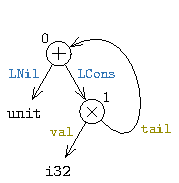
\includegraphics[scale=1.3]{chapters/figures/figTypeTreeList1.pdf}
\end{center}
\vspace{30px}
\caption{\label{fig:typetreelist1}\cons{List} = \cons{LNil} | \newline \cons{LCons}(\type{i32}, \type{List})}
\end{subfigure}%
&
\begin{subfigure}[b]{0.33\textwidth}
\begin{center}
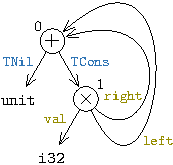
\includegraphics[scale=1.3]{chapters/figures/figTypeTreeTree1.pdf}
\end{center}
\vspace{35px}
\caption{\label{fig:typetreetree1}\cons{Tree} = \cons{TNil} | \newline \cons{TCons}(\type{i32}, \type{Tree}, \type{Tree})}
\end{subfigure}%
&
\begin{subfigure}[b]{0.33\textwidth}
\begin{center}
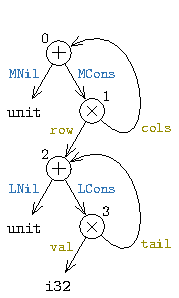
\includegraphics[scale=1.3]{chapters/figures/figTypeTreeMatrix1.pdf}
\end{center}
\caption{\label{fig:typetreematrix1}\cons{Matrix} = \cons{MNil} | \newline \cons{MCons}(\type{List}, \type{Matrix})}
\end{subfigure}%
\\
\end{tabular}
\caption{\label{fig:typetrees}Type trees for the ADTs \type{List}, \type{Tree} and \type{Matrix} respectively.}
\end{figure}

\Cref{fig:typetrees} shows the type trees for three ADTs -- \type{List}, \type{Tree}, and \type{Matrix} respectively.
In a type tree, each internal node represents either a product (\prodn{}) or a sum (\sumn{}) type constructor.
The leaf nodes are the scalar types.
Each outgoing edge of a \sumn{} node is associated with a data constructor of the corresponding ADT (i.e. \cons{LCons} for \type{List}).
Similarly, each outgoing edge of a \prodn{} node is associated with a field of the corresponding data constructor (i.e. \field{val} for \type{LCons}).
We assign integer indices to the internal nodes and use \ttedge{v}{label}\footnote{
The \ttedge{v}{label} syntax is chosen over $v_1 \rightarrow v_2$ because
type trees may have multi-edges (e.g. \cref{fig:typetreetree1}), in which case
$v_1 \rightarrow v_2$ no longer represents an unique edge.}
to identify the edge outgoing at $v$ associated with {\tt label},
where {\tt label} is either a data constructor or a field name.
The root node is denoted by $v_0$.
The edges going outward from the root node are called {\em tree-edges}, e.g., \ttedge{0}{LCons} and \ttedge{1}{val} in \cref{fig:typetreelist1}.
Edges that are not tree-edges, are called {\em backedges}, e.g., \ttedge{1}{cols} in \cref{fig:typetreematrix1}.
Every backedge induces an unique simple cycle in the type tree representation.

\begin{figure}[H]
\begin{tabular}{@{}c@{}c@{}c@{}}
\begin{subfigure}[b]{0.30\textwidth}
\begin{center}
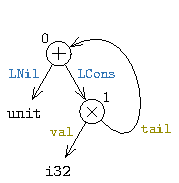
\includegraphics[scale=1.3]{chapters/figures/figTypeTreeList1.pdf}
\end{center}
\vspace{30px}
\caption{\label{fig:typetreelistpeel1} Canonical \type{List} ADT}
\end{subfigure}%
&
\begin{subfigure}[b]{0.33\textwidth}
\begin{center}
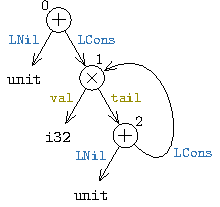
\includegraphics[scale=1.3]{chapters/figures/figTypeTreeList2.pdf}
\end{center}
\vspace{20px}
\caption{\label{fig:typetreelistpeel2} Peeled \type{List} ADT}
\end{subfigure}%
&
\begin{subfigure}[b]{0.33\textwidth}
\begin{center}
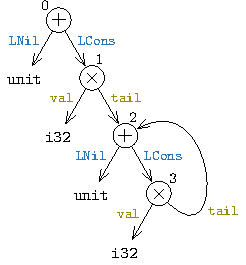
\includegraphics[scale=1.3]{chapters/figures/figTypeTreeList3.pdf}
\end{center}
\caption{\label{fig:typetreelistpeel3} Unrolled \type{List} ADT}
\end{subfigure}%
\\
\end{tabular}
\caption{\label{fig:typetreespeel}Three equivalent graphical representations for \type{List} ADT.
\Cref{fig:typetreelistpeel1} shows the graphical representation of the canonical form of \type{List}.
\Cref{fig:typetreelistpeel2} is obtained by peeling the {\em backedge} [2,1] in \cref{fig:typetreelistpeel1}.
\Cref{fig:typetreelistpeel3} is obtained by unrolling the backedge [2,1] in \cref{fig:typetreelistpeel1} or by
peeling the backedge [4,1] in \cref{fig:typetreelistpeel2} respectively.}
\end{figure}

Recall that types in \SpecL{} (and in IR) follow equirecursive typing rules i.e. types
$\mu \alpha. T$ and $T[\mu \alpha. T/\alpha]$ in \typegrammar{} are {\em equal} types,
where $T[\mu \alpha. T/\alpha]$ represents the new type obtained by substituting all free
instances of $\alpha$ with $\mu \alpha. T$, and is defined as the {\em unfolding} of $\mu \alpha. T$.
In general, under equirecursive typing, two types are equal iff their infinite expansions (through unfolding) are equal.
In the type tree representation, two types are equal iff their infinite expansions are equal.
Such type trees are called isomorphic and two types are isomorphic iff they represent the same type.
An unfolding in the term representation corresponds to {\em unrolling} one iteration of a simple cycle in its type tree.
\Cref{fig:typetreespeel} shows three type trees for the \type{List} type.
\Cref{fig:typetreelistpeel1} corresponds to the canonical (intuitively the `smallest') type tree for the \type{List} type.
The type trees \cref{fig:typetreelistpeel2,fig:typetreelistpeel3} are obtained by {\em peeling} and unrolling
the backedge \ttedge{1}{tail} (in \cref{fig:typetreelistpeel1}) respectively.
Peeling is a form of partial unrolling which only extracts the head of a cycle.
In practice, equality of two types (encoded in \typegrammar{}) can be reposed as syntactic
equality of their {\em canonical forms} \cite{canonicalrecursivetypes}.
In general, type trees may contain cycles (due to backedges) and hence are not quite `trees'.
However, they represent the actual (possibly infinite) trees obtained through repeated unrolling of cycles.

\begin{figure}[H]
\begin{tabular}{cc}
\begin{subfigure}[b]{0.45\textwidth}
\begin{center}
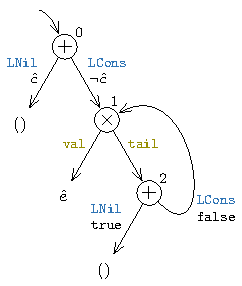
\includegraphics[scale=1.4]{chapters/figures/figValueTreeList1.pdf}
\end{center}
\caption{\label{fig:valuetreelist1}\sumIf{c} \sumThen{\cons{LNil}} \sumElse{\cons{LCons}(e, \cons{LNil})}}
\end{subfigure}%
&
\begin{tabular}{@{}c@{}}
\begin{subfigure}[b]{0.53\textwidth}
\begin{center}
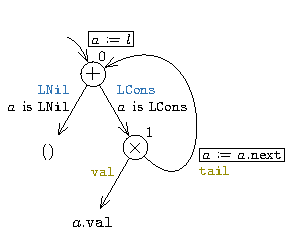
\includegraphics[scale=1.3]{chapters/figures/figValueTreeVarList.pdf}
\end{center}
\caption{\label{fig:valuetreevarlist}$l\ctype{List}$}
\end{subfigure}%
\\
\begin{subfigure}[b]{0.53\textwidth}
\begin{center}
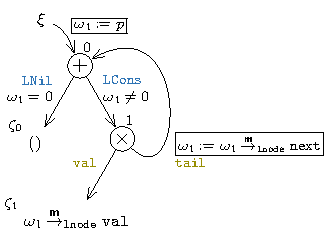
\includegraphics[scale=1.3]{chapters/figures/figValueTreeClist.pdf}
\end{center}
\caption{\label{fig:valuetreeclist}\lifted{list}{\mem{}}{lnode}{p}}
\end{subfigure}%
\\
\end{tabular}
\\
\end{tabular}
\caption{\label{fig:valuetrees}Value trees for three \type{List}-typed expressions.}
\end{figure}

With type trees out of the way, we are ready to present their value analogue called `value trees'.
\Cref{fig:valuetrees} shows the value trees for three \type{List} expressions.
Note that, all three value trees are isomorphic to one of the
\type{List} type trees shown in \cref{fig:typetreespeel}, e.g.,
\cref{fig:valuetreelist2} is isomorphic to \cref{fig:typetreelistpeel2}.
In general, for an expression $e$ of type $\tau$, its value tree $\mathcal{V}(e)$ resembles
a type tree $\mathcal{T}(\tau)$ with the following distinctions:

\begin{enumerate}
\item Similar to a type tree, each internal node in $\mathcal{V}(e)$ is either a \sumn{} or a \prodn{} node.
\item Each node $v$ in $\mathcal{V}(e)$ is associated with a symbolic state $\Omega_v$
similar to the control-flow graph representation (presented in \cref{sec:cfg}) of a program.
\item Recall that an edge leaving a \sumn{} node is labeled with a data constructor.
These edges are additionally labeled with an {\em edge condition} (a boolean valued function over $\Omega_n$).
We identify such an edge with \vtedge{v}{\mathnormal{V}}{c}, where $v$ is the \sumn{} node,
$V$ is a data constructor and $c$ is the edge condition.
The set of edge conditions of all edges leaving a \sumn{} node must be mutually exclusive and exhaustive.
\item Recall that an edge $v \rightarrow v'$ leaving a \prodn{} node is labeled with a field name.
Such an edge is also associated with a transfer function ($\Omega_{v'}$ as a function of $\Omega_v$),
and is denoted by \vtedge{v}{fi}{\xfer{}}, where $v$ is the \prodn{} node,
\field{fi} is a field name and \xfer{} is the transfer function.
\item Instead of a scalar type $\tau_s$, each leaf node $v$ in $\mathcal{V}(e)$ contains an expression
of type $\tau_s$ (as a function of $\Omega_{v}$).
\item Additionally, a value tree contains a special node (called the {\em entry node}), and a special edge
(called the {\em entry edge}) from the entry node to $v_0$ (i.e. the root of the tree).
We use $\xi$ to denote the entry node.
The entry edge is associated with a transfer function $\xfer{}_\xi$.
We often omit the entry node in figures for brevity.
\item A value tree $\mathcal{V}(e)$ can be converted to a type tree $\mathcal{T}$ as follows:
(a) remove the entry node and edge pair, (b) remove edge conditions and transfer functions
associated with all edges, and (c) replace each leaf node expression of (scalar) type $\tau_s$
with $\tau_s$ itself.
The resulting type tree $\mathcal{T}$ represents the type $\tau$ of the expression $e$.
\end{enumerate}

Intuitively, a value tree simultaneously represents the value of the expression as well as
the canonical CFG of its deconstruction program.
We will subsequently discuss these properties along with their applications in the context
of our proof discharge algorithm.
First, we give an algorithm to convert an expression $e$ to its value tree representation $\mathcal{V}(e)$.

\subsection{Conversion of Expressions to their Value Trees}
\label{sec:valuetreeconv}
In this section, we present an algorithm to recursively construct a value tree for any arbitrary expression $e$.
We take a visual approach to align with the graphical nature of value trees.

\begin{figure}[H]
\begin{subfigure}[b]{\textwidth}
\begin{center}
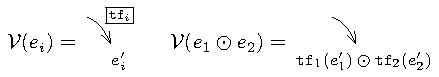
\includegraphics[scale=1.3]{chapters/figures/figValueTreeConvScalar.pdf}
\end{center}
\end{subfigure}
\caption{\label{fig:valuetreeconvscalar} Construction of $\mathcal{V}(e_1 \odot e_2)$ from $\mathcal{V}(e_1)$ and $\mathcal{V}(e_2)$.\\
$\odot$ represents an arbitrary scalar operator.}
\end{figure}

\subsubsection{Scalar Operators}
Given an expression $e = e_1 \odot e_2$,
\cref{fig:valuetreeconvscalar} shows the construction of $\mathcal{V}(e)$
from $\mathcal{V}(e_1)$ and $\mathcal{V}(e_2)$ respectively.
Since $e_1$ and $e_2$ have scalar types, their value trees must have exactly one
node (i.e. a leaf node) containing an expression ($e'_1$ and $e'_2$ respectively) of the same type.
$\odot$ represents an aribtrary scalar operator, i.e. an operator that accepts
scalar values and produce another scalar value.
Importantly, arrays over bitvectors are considered scalar types and thus
memory load and store satisfy the properties of scalar operators.
Given an expression $s$ and a transfer function \xfer{}, $\xfer{}(s)$
represents the expression obtained by applying \xfer{}, interpreted as a substitution,
to $s$. This is equivalent to the weakest-precondition of $s$ along an edge associated
with \xfer{}.
The construction shown in \cref{fig:valuetreeconvscalar} can be generalized to
$n$-ary scalar operators for $n>2$.

\begin{figure}[H]
\begin{subfigure}[b]{\textwidth}
\begin{center}
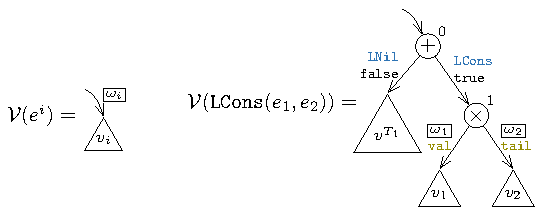
\includegraphics[scale=1.3]{chapters/figures/figValueTreeConvCons.pdf}
\end{center}
\end{subfigure}
\caption{\label{fig:valuetreeconvcons} Construction of $\mathcal{V}(\cons{LCons}(e_1,e_2))$ from $\mathcal{V}(e_1)$ and $\mathcal{V}(e_2)$.\\
$\mathcal{R}_\cons{LNil}$ represents an arbitrary value tree corresponding to the product-type (in \typegrammar{}) associated with \cons{LNil}.}
\end{figure}

\subsubsection{ADT Data Constructors}
Given an expression $e = \cons{LCons}(e_1, e_2)$,
\cref{fig:valuetreeconvcons} depicts the construction of $\mathcal{V}(e)$
from $\mathcal{V}(e_1)$ and $\mathcal{V}(e_2)$ respectively.
In general, for an arbitrary data constructor $V$ of ADT $T$,
the construction begins with a \sumn{} node (0 in \cref{fig:valuetreeconvcons})
such that the outgoing edge associated with the value constructor $V$ (\cons{LCons} in \cref{fig:valuetreeconvcons})
has an edge condition of {\tt true} while all other edges are assigned the edge condition {\tt false}.
For each data constructor $V' \neq V$ of $T$, we append a random value tree corresponding to the product-type
associated with $V'$ in \typegrammar{}.
For example, given \type{List} is associated with the sum-type $\mu \alpha. \type{Unit} + (\type{i32} \times \alpha)$,
the product-types associated with \cons{LNil} and \cons{LCons} are:
$\type{Unit}$ and $\mu \alpha. \type{i32} \times (\type{Unit} + \alpha)$ respectively.
We use $\mathcal{R}_\tau$ to denote an arbitrary (i.e. random) value tree of type $\tau$.
For the outgoing edge associated with the data constructor $V$ (\vtedge{0}{LCons}{\tt true} in \cref{fig:valuetreeconvcons}),
we construct a product node (1 in \cref{fig:valuetreeconvcons}) and append the
value trees corresponding to the arguments $e_i$ as children of the product node.
% Interpreted as a program, all random value trees are appended under a {\tt false} edge condition
% (i.e. unreachable) and hence do not change the value represented by $\mathcal{V}(e)$.
% Their only responsibility is to keep the overall structure of $\mathcal{V}(e)$ isomorphic to $\mathcal{T}(\type{List})$.

\begin{figure}[H]
\begin{subfigure}[b]{\textwidth}
\begin{center}
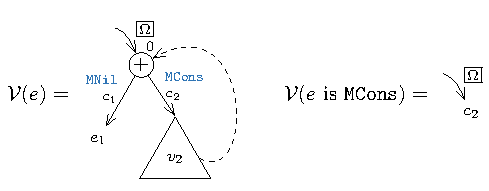
\includegraphics[scale=1.3]{chapters/figures/figValueTreeConvSumIs.pdf}
\end{center}
\end{subfigure}
\caption{\label{fig:valuetreeconvsumis} Construction of $\mathcal{V}(\sumIs{e}{MCons})$ from $\mathcal{V}(e)$.\\
The dashed edge represents the (possibly empty) set of backedges originating in the subtree rooted at $v_2$ that terminates at 0.}
\end{figure}

\subsubsection{Sum-Is Operator}
Given a {\em sum-is} expression $e' = \sumIs{e}{MCons}$,
\cref{fig:valuetreeconvsumis} shows the construction of $\mathcal{V}(e')$
from $\mathcal{V}(e)$.
The process is rather straightforward and for a general expression $\sumIs{e}{\mathnormal{V}_i}$, entails extracting the
edge condition $c$ ($c_2$ in \cref{fig:valuetreeconvsumis}) from $\mathcal{V}(\sumIs{e}{\mathnormal{V}_i})$ edge
\vtedge{v_0}{\mathnormal{V}}{c} (\vtedge{0}{MCons}{c_2} in \cref{fig:valuetreeconvsumis}).
Notice that the entry transfer function $\xfer{}$ is preserved during this construction.

\begin{figure}[H]
\begin{subfigure}[b]{\textwidth}
\begin{center}
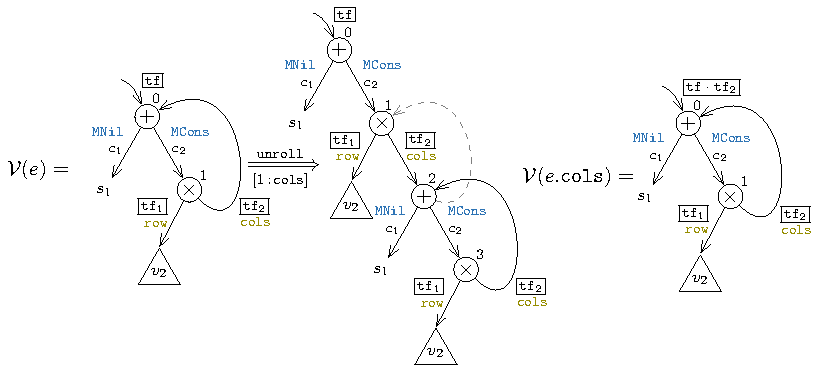
\includegraphics[scale=1.2]{chapters/figures/figValueTreeConvProdAccess.pdf}
\end{center}
\end{subfigure}
\caption{\label{fig:valuetreeconvprodaccess} Construction of $\mathcal{V}(\prodAccess{e}{cols})$ from $\mathcal{V}(e)$.\\
Similar to type trees, {\tt unroll} \ttedge{1}{cols} represents the operation of hoisting one iteration of the cycle \pathset{0,1,0}.}
\end{figure}

\subsubsection{Product-Access Operator}
Given an expression $e' = \prodAccess{e}{cols}$,
\cref{fig:valuetreeconvprodaccess} depicts the construction of $\mathcal{V}(e')$
from $\mathcal{V}(e)$.
Intuitively, $\mathcal{V}(e')$ represents the subtree of $\mathcal{V}(e)$ rooted at the \sumn{} node reached by taking
the edges \vtedge{0}{MCons}{c_2} followed by \vtedge{1}{cols}{\xfer{}_2}.
However, this path may contain backedges or the subtree itself may contain backedges leaving the subtree.
In such a case, we perform peeling until all such backedges strickly terminate within this subtree.
For example, in \cref{fig:valuetreeconvprodaccess}, the edge \vtedge{1}{cols}{\Omega_2} is a backedge and hence we peel it once.
In the resulting (equivalent) value tree, the subtree (rooted at 2) contains a backedge leaving the subtree (dashed edge \ttedge{2}{MCons})
which requires one more peeling operation.
The resulting value tree contains the subtree rooted at the \sumn{} node 2 which satisfies the two conditions above and
hence $\mathcal{V}(e')$ is simply constructed by extracting the subtree rooted at node 2.
Note that we preserve the transfer functions from the entry to node 2 during extraction.
$\xfer{}_1 \cdot \xfer{}_2$ represents the composition of the transfer functions $\xfer{}_1$ and $\xfer{}_2$ respectively.

\begin{figure}[H]
\begin{subfigure}[b]{\textwidth}
\begin{center}
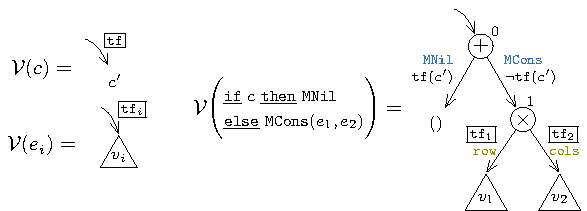
\includegraphics[scale=1.3]{chapters/figures/figValueTreeConvIte.pdf}
\end{center}
\end{subfigure}
\caption{\label{fig:valuetreeconvite} Construction of $\mathcal{V}($ \sumIf{c} \sumThen{\cons{MNil}} \sumElse{\cons{MCons}(e_1,e_2)} $)$ from $\mathcal{V}(c)$, $\mathcal{V}(e_1)$ and $\mathcal{V}(e_2)$.}
\end{figure}

\subsubsection{\underline{If}-\underline{Then}-\underline{Else} Operator}
Given an expression $e =$ \sumIf{c} \sumThen{\cons{MNil}} \sumElse{\cons{MCons}(e_1,e_2)},
\cref{fig:valuetreeconvite} describes the construction of $\mathcal{V}(e)$
using $\mathcal{V}(c)$, $\mathcal{V}(e_1)$ and $\mathcal{V}(e_2)$.
Let us consider a general \sumDtor{} expression $e$ (associated with the ADT $T$ with data constructors $V_1,V_2,\dots,V_n$)
such that the branch associated with $V_i$ is given by $V_i(e_i^1,e_i^2,\dots)$.
We begin with the construction of a \sumn{} root node (0 in \cref{fig:valuetreeconvite})
such that the outgoing edge associated with $V_i$ has the edge condition equal to the
expression path condition of the branch $V_i(e_i^1,e_i^2,\dots)$
($\xfer{}(c')$ and $\neg \xfer{}(c')$ for \cons{MNil} and \cons{MCons} respectively in \cref{fig:valuetreeconvite}).
For each outgoing edge associated with the data constructor $V_i$, we construct a \prodn{} node
(1 for \cons{MCons} in \cref{fig:valuetreeconvite}) and append the value trees corresponding to
the arguments $e_i^j$ as its children.

\begin{figure}[H]
\begin{subfigure}[b]{\textwidth}
\begin{center}
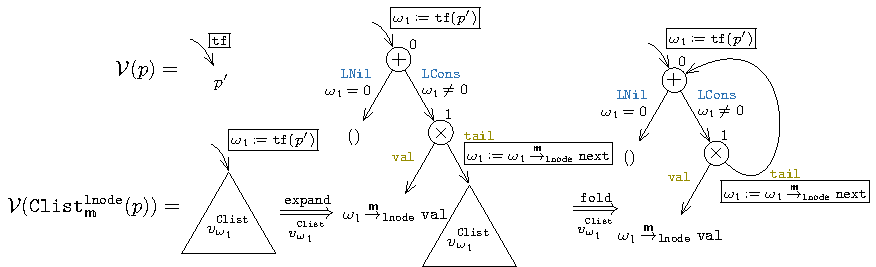
\includegraphics[scale=1.2]{chapters/figures/figValueTreeConvLift.pdf}
\end{center}
\end{subfigure}
\caption{\label{fig:valuetreeconvlift} Construction of $\mathcal{V}(\lifted{list}{\mem{}}{lnode}{p})$ from $\mathcal{V}(p)$.\\
The process involves assuming that $v_\vtse{1}^\lift{list}{}{}$ is the value tree of $\lifted{list}{\mem{}}{lnode}{\vtse{1}}$,
followed by expansion of $v_\vtse{1}^\lift{list}{}{}$ using the definition of \lift{list}{\mem{}}{lnode} (in \cref{eqn:clist})
and, finally folding the tree-edge \ttedge{1}{tail} incident on the self-referencial subtree $v_\vtse{1}^\lift{list}{}{}$ into a backedge.}
\end{figure}

\subsubsection{Lifting Constructor}
Given an expression $e = \lifted{list}{\mem{}}{lnode}{p}$,
\cref{fig:valuetreeconvlift} shows the construction of $\mathcal{V}(e)$
from $\mathcal{V}(p)$.
Recall the recursive definition of the lifting constructor \lift{list}{\mem{}}{lnode} given in
\cref{eqn:clist}.
We start by assuming that $v_\vtse{1}^\lift{list}{}{}$ is the value tree for the lifted expression
\lifted{list}{\mem{}}{lnode}{\vtse{1}}.
Hence, the value tree of \lifted{list}{\mem{}}{lnode}{p} is identical to $v_\vtse{1}^\lift{list}{}{}$
except we assign the actual argument (i.e. $\xfer{}(p')$) to the formal argument $\vtse{1}$ along the
entry edge.
Next, we expand the subtree $v_\vtse{1}^\lift{list}{}{}$ based on the unrolling procedure of \lift{list}{\mem{}}{lnode}
(defined in \cref{eqn:clist}) until the entire value tree becomes a self-referencial structure.
For example, after expanding through \cref{eqn:clist} once in \cref{fig:valuetreeconvlift},
the value tree contains a tree-edge \ttedge{1}{tail} incident on the self-referencial subtree $v_\vtse{1}^\lift{list}{}{}$.
In the last step, we fold all self-referencial tree-edges (\ttedge{1}{tail} in \cref{fig:valuetreeconvlift})
by converting them into backedges terminating at the root of the subtree being referenced
(0 for $v_\vtse{1}^\lift{list}{}{}$ in \cref{fig:valuetreeconvlift}).

\begin{figure}[H]
\begin{subfigure}[b]{\textwidth}
\begin{center}
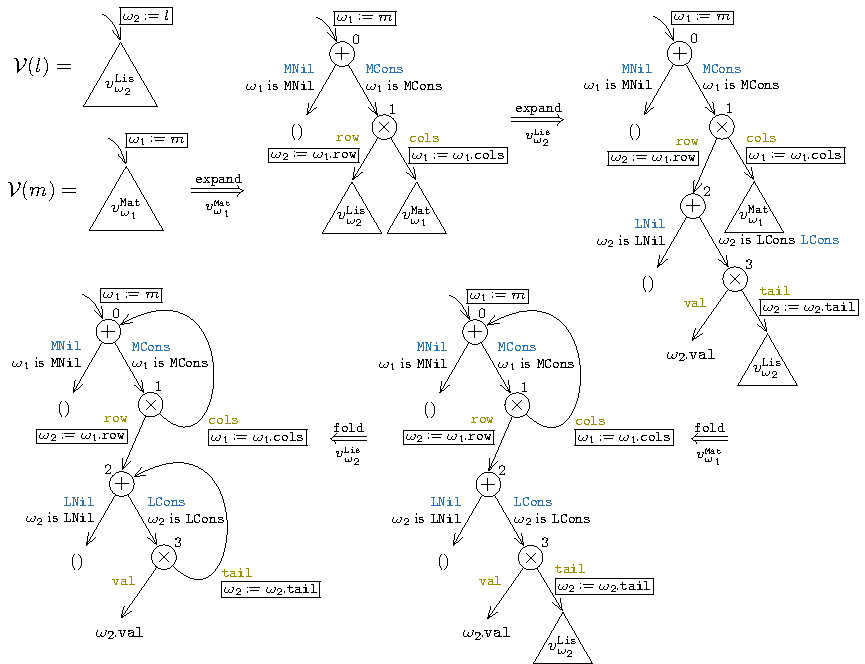
\includegraphics[scale=1.2]{chapters/figures/figValueTreeConvVar.pdf}
\end{center}
\end{subfigure}
\caption{\label{fig:valuetreeconvvar} Construction of $\mathcal{V}(m)$ for a \type{Matrix} variable $m$.
The process is analogous to the construction of value trees for lifted expressions as shown in \cref{fig:valuetreeconvlift}.}
\end{figure}

\subsubsection{Variables}
Finally, we are interested in constructing the value tree for a variable.
Recall that, every ADT (pseudo-)variable is associated with an unrolling procedure
characterized by the ADT itself, e.g., \cref{eqn:specDeconstruct}
for the \type{List} variable $l$.
The \type{Matrix} ADT is defined as
$\type{Matrix} = \cons{MNil} \ | \ \cons{MCons}(\type{List},\type{Matrix})$,
and thus the unrolling procedure for a \type{Matrix} variable $m$ is given by:

\begin{equation}
\label{matrixunrollingprocedure}
m = \sumIf{\sumIs{m}{MNil}} \  \sumThen{\cons{MNil}} \  \sumElse{\cons{MCons}(\prodAccess{m}{row}, \prodAccess{m}{cols})}
\end{equation}

\Cref{fig:valuetreeconvvar} illustrates the construction $\mathcal{V}(m)$ for the \type{Matrix} variable $m$.
The process consists of the same three steps used to construct the value tree
for a lifted expression -- assume, expand and fold.
First, we assume that $v_\vtse{1}^\type{Mat}$ and $v_\vtse{2}^\type{Lis}$ are the value trees
corresponding to the pseudo-variables \vtse{1} and \vtse{2} of \type{Matrix} and \type{List}
types respectively.
Thus, $\mathcal{V}(m)$ is equal to $v_\vtse{1}^\type{Mat}$ except for $\xfer{}_\xi = \{ \vtse{1} \mapsfrom m \}$.
We expand the definitions of $v_\vtse{1}^\type{Mat}$ and $v_\vtse{2}^\type{Lis}$ once each before
the value tree becomes self-referencial.
Finally, we fold the tree-edges \ttedge{1}{cols} and \ttedge{3}{tail} into the backedges
terminating at the roots of the subtrees representing $v_\vtse{1}^\type{Mat}$ and $v_\vtse{2}^\type{Lis}$
respectively (nodes 0 and 3 in \cref{fig:valuetreeconvvar}).

\subsection{Applications of Value Trees}
\label{sec:valuetreeapps}
With the conversion algorithm out of the way, we next discuss a handful of properties of value trees along with
their applications, in the context of our proof discharge algorithm.
This allows us to formulate the value tree construction algorithms for approximate \recursiveRelations{}.

\subsubsection{Program Interpretation of Value Trees}
\label{sec:valuetreeasprog}
A value tree $\mathcal{V}$ can be interpreted as a {\em non-deterministic} Control-Flow Graph corresponding to a program.
Similar to the CFG representation, every node $v$ is associated with a symbolic state $\Omega_n$.
In this interpretation, edges without an edge condition (e.g. outgoing at a \prodn{} node) are assigned the {\tt true}
edge condition. Similarly, edges without a transfer function (e.g. outgoing at a \sumn{} node) are assigned an
identity transfer function.
The entry node $\xi$ is the start node and each leaf node $\zeta$ represents an exit node.
An edge incident on a leaf node $\zeta$ (containing an expression $e$) is called an exit edge and is associated
with an observable action that returns $e$.

\begin{figure}[t!]
\begin{tabular}{@{\hskip 2mm}c@{}c@{}}
\begin{subfigure}[b]{0.5\textwidth}
\begin{center}
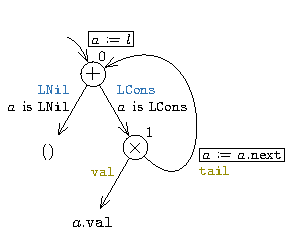
\includegraphics[scale=1.35]{chapters/figures/figValueTreeVarList.pdf}
\end{center}
\vspace{4px}
\caption{\label{fig:valuetreevar}$\mathcal{V}(l)$}
\end{subfigure}%
&
\begin{subfigure}[b]{0.5\textwidth}
\begin{center}
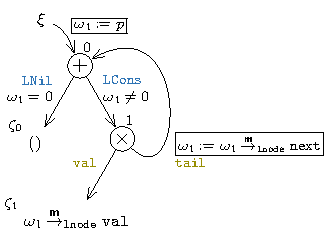
\includegraphics[scale=1.35]{chapters/figures/figValueTreeClist.pdf}
\end{center}
\caption{\label{fig:valuetreelifted}$\mathcal{V}(\lifted{list}{\mem{}}{lnode}{p})$}
\end{subfigure}%
\\
\end{tabular}
\caption{\label{fig:valuetreeapproxeg}Value trees for a \type{List} variable $l$ and a lifted expression \lifted{list}{\mem{}}{lnode}{p} respectively.}
\end{figure}

\subsubsection{Canonical Deconstruction Property}
\label{sec:valuetreecanonicaldecons}
A path originating at the entry node $\xi$ and terminating at an exit node $\zeta$ is called an
{\em execution path} and is denoted by $\execpath{}$.
Generalizing the edge syntax, $\ttedge{v}{label_1,label_2,\dots ,label_n}$ represents the path
starting at $v$ such that its $n$ consecutive edges are associated with the labels ${\tt label}_i \forall i \in [1,n]$.
Hence, an execution path \execpath{} can be written as $\xi \rightarrow \ttedge{v_0}{label_1,label_2,\dots ,label_n}$,
or $\execpath{}[{\tt label_1,label_2,\dots,label_n}]$ in short.
Recall that, edges leaving a \prodn{} node are associated with field names.
The {\em field trace of \execpath{}}, $\ftrace{\execpath{}}$ is defiend as the ordered list of field names associated with edges in the path \execpath{}.
For an execution path $\execpath{}[\cons{LCons},\field{tail},\cons{LCons},\field{val}]$ in the value tree shown in \cref{fig:valuetreevar},
$\ftrace{\execpath{}}$ is given by $[\field{tail},\field{val}]$.
Given a value tree $\mathcal{V}(e)$ and an execution path $\execpath{}$ with a field trace $[{\tt a_1,a_2,\dots,a_n}]$,
$\prodAccess{e}{a_1,a_2,.,a_n}$ is defined as the component of $e$ with respect to $\execpath{}$, denoted by $\comp{e}{\execpath{}}$.
The {\em canonical deconstruction property} for a value tree ensures that:

\begin{enumerate}
\item The condition under which $\comp{e}{\execpath{}}$ is accessible (i.e. is well-formed as discussed in \cref{sec:irconv})
is equal to the path condition of $\execpath{}$, denoted by $\pathcond{\execpath{}}$.
\item The value of $\comp{e}{\execpath{}}$ is equal to the value returned by $\mathcal{V}(e)$ (interpreted as a program) along the
execution path $\execpath{}$. This is equivalent to the weakest-precondition of the value returned along the path $\execpath{}$
and is denoted by $\retval{\execpath{}}$.
\item Both $\pathcond{\execpath{}}$ and $\retval{\execpath{}}$ are in the canonical form (\cref{sec:canonicalalgo}).
\end{enumerate}

Consider the value tree corresponding to the lifted expression $e=\lifted{list}{\mem{}}{lnode}{p}$ as shown in \cref{fig:valuetreelifted}.
The execution path $\execpath{}[\cons{LCons},\field{val}]$ corresponds to the component $\comp{e}{\execpath{}} = \prodAccess{\lifted{list}{\mem{}}{lnode}{p}}{val}$.
The path condition and the value returned along $\execpath{}$ are given by $\pathcond{\execpath{}} = (p \neq 0)$ and
$\retval{\execpath{}} = \structPointer{p}{\mem{}}{lnode}{val}$ respectively.
Note that $\comp{e}{\execpath{}}$ is well-formed iff $\pathcond{\execpath{}}$ is true and
$\comp{e}{\execpath{}} = \retval{\execpath{}}$.
Furthermore, both are in canonical forms.

\subsubsection{Reduction of Approximate Recursive Relations}
\label{sec:valuetreeapprox}
Since an ADT represents a `sum of product' type, each level of an ADT value
(in its expression tree as shown in \cref{sec:adtdepth}) corresponds to two levels -- \sumn{} and \prodn{}
in the value tree representation.
Combining the above observation with the value tree properties discussed above (\cref{sec:valuetreeasprog,sec:valuetreecanonicaldecons})
allow us to reformulate approximate \recursiveRelations{} between $l_1$ and $l_2$ as {\em bounded} equivalence \cite{boundedmodelchecking}
between $\mathcal{V}(l_1)$ and $\mathcal{V}(l_2)$.
The $d$-depth over-approximation $l_1 \indEqDepth{d} l_2$ asserts that $\mathcal{V}(l_1)$ and $\mathcal{V}(l_2)$ are equivalent
for all execution paths up to a depth\footnote{
The depth of an execution path \execpath{} is defined as the depth of the exit node in the unrolled (executable) value tree.
If \execpath{} contains $n$ edges (including the entry edge), then its depth is equal to $(n-1)$.} of $2 \cdot d$ .
Clearly, this is a weaker condition because $\mathcal{V}(l_1)$ and $\mathcal{V}(l_2)$ may behave differently for longer execution paths.
The $d$-depth under-approximation $l_1 \indEqUapprox{d} l_2$ asserts that $\mathcal{V}(l_1)$ and $\mathcal{V}(l_2)$ are equivalent for
all execution paths up to a depth of $2 \cdot d$ and all other execution paths are unreachable.
This is a stronger condition than general equivalence because paths deeper than $2 \cdot d$ may indeed be reachable.
Let $\execpaths{\delta}{l_1}{l_2}$ be the set of all execution path pairs $\langle \execpath{}_1, \execpath{}_2 \rangle$ in $l_1$ and $l_2$,
such that $\ftrace{\execpath{}_1} = \ftrace{\execpath{}_2}$ and depths of $\execpath{}_1$ and $\execpath{}_2$ are equal to $\delta$.
For example, consider the value trees shown in \cref{fig:valuetreeapproxeg} corresponding to the \type{List} values
$e_1 = l$ and $e_2 = \lifted{list}{\mem{}}{clnode}{p}$ respectively.
Then, $\execpaths{0}{e_1}{e_2} = \emptyset$, $\execpaths{1}{e_1}{e_2} = \{ \langle \pathset{\xi,0,\zeta_0},\pathset{\xi,0,\zeta_0} \rangle \}$
and $\execpaths{2}{e_1}{e_2} = \{ \langle \pathset{\xi,0,1,\zeta_1},\pathset{\xi,0,1,\zeta_1} \rangle \}$.
Finally, the $d$-depth approximations of $l_1 \indEq{} l_2$ are given by:

\begin{equation}
\label{eqn:valuetreeapprox}
\begin{footnotesize}
\begin{aligned}
l_1 \indEqDepth{d} l_2 &= \sum_{\delta=0}^{2 \cdot d} \Bigg( \bigwedge_{\substack{\langle \execpath{}_1, \execpath{}_2 \rangle \\ \in \execpaths{\delta}{l_1}{l_2}}} \begin{array}{@{}c@{}} \pathcond{\execpath{}_1} = \pathcond{\execpath{}} \\ \retval{\execpath{}_1} = \retval{\execpath{}_2} \end{array} \Bigg) \\
l_1 \indEqUapprox{d} l_2 &= \sum_{\delta=0}^{2 \cdot d} \Bigg( \bigwedge_{\substack{\langle \execpath{}_1, \execpath{}_2 \rangle \\ \in \execpaths{\delta}{l_1}{l_2}}} \begin{array}{@{}c@{}} \pathcond{\execpath{}_1} = \pathcond{\execpath{}} \\ \retval{\execpath{}_1} = \retval{\execpath{}_2} \end{array} \Bigg) \land \Bigg( \bigwedge_{\substack{\langle \execpath{}_1, \execpath{}_2 \rangle \\ \in \execpaths{2 \cdot d + 1}{l_1}{l_2}}} \begin{array}{@{}c@{}} \neg \pathcond{\execpath{}_1} \\ \neg \pathcond{\execpath{}_2} \end{array} \Bigg)
\end{aligned}
\end{footnotesize}
\end{equation}

Recall that the canonical deconstruction property ensures that the reductions in \cref{eqn:valuetreeapprox} are in the canonical form.
Thus, the value trees corresponding to $l_1 \indEqDepth{d} l_2$ and $l_1 \indEqUapprox{d} l_2$ are constructed by creating a single (leaf) node
with the boolean expressions given in \cref{eqn:valuetreeapprox}.
The conversion algorithm presented in \cref{sec:valuetreeconv} together with the handling of approximate \recursiveRelations{} described above
enables the reduction of a proof obligation $P$ without \recursiveRelations{} directly to its canonical form by --
(a) constructing $\mathcal{V}(P)$ and (b) extracting the boolean expression at its root.

\subsubsection{Bisimilarity of Value Trees}
\label{sec:valuetreebisim}
Unlike its approximations, a \recursiveRelation{} $l_1 \indEq{} l_2$ asserts general equivalence between
$\mathcal{V}(l_1)$ and $\mathcal{V}(l_2)$ respectively.
Similar to our top-level equivalence check between \sprog{} and \cprog{},
we attempt to prove that $\mathcal{V}(l_1)$ and $\mathcal{V}(l_2)$ are bisimilar.
To make the search for a bisimulation relation easier, we peel $\mathcal{V}(l_1)$ and $\mathcal{V}(l_2)$
to unify their static structures.
Once unified, the bisimulation relation requires the inference of inductive invariants at correlated nodes such that
under the precondition at $(\xi\!:\!\xi)$, inductive invariants hold and both $\mathcal{V}(l_1)$ and $\mathcal{V}(l_2)$
have equal observables at correlated exit nodes $(\zeta_i\!:\!\zeta_i)$.

\begin{figure}[t!]
\begin{tabular}{@{}c@{}}
\begin{subfigure}[b]{0.5\textwidth}
\begin{center}
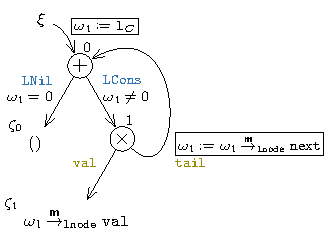
\includegraphics[scale=1.25]{chapters/figures/figValueTreeClistm.pdf}
\end{center}
\caption{\label{fig:valuetreeclistm}$\mathcal{V}(\lifted{list}{\mem{}}{lnode}{\cv{l}})$}
\end{subfigure}%
\begin{subfigure}[b]{0.5\textwidth}
\begin{center}
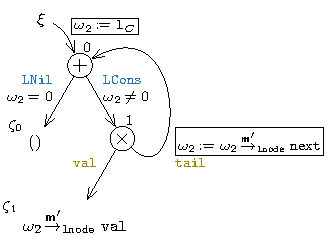
\includegraphics[scale=1.25]{chapters/figures/figValueTreeClistmdash.pdf}
\end{center}
\caption{\label{fig:valuetreeclistmdash}$\mathcal{V}(\lifted{list}{\mem{}'}{lnode}{\cv{l}})$}
\end{subfigure}%
\\
\begin{subfigure}[b]{\textwidth}
\begin{center}
\begin{footnotesize}
\begin{tabular}{@{\hskip 5mm}cl@{\hskip 8mm}l@{\hskip 8mm}l@{\hskip 3mm}}
\toprule
{\bf Node Pair} & \multicolumn{3}{c}{\bf Invariants} \\
\toprule
$(\xi \!:\! \xi)$ & \multicolumn{3}{l}{$\circled{\small P} \  \lhs{}$ in \cref{eqn:cat3revisit}} \\
\midrule
\multirow{3}{*}{\makecell[c]{$(0 \!:\! 0)$ \\ $(1 \!:\! 1)$ }} & $\circled{\footnotesize I1} \  \vtse{1} = \vtse{2}$ & $\circled{\footnotesize I2} \  \vtse{1} \pointsTo{} \{ \mlrs{\cpc{4}}, \heapr \}$ & $\circled{\footnotesize I3} \  \vtse{2} \pointsTo{} \{ \mlrs{\cpc{4}}, \heapr \}$ \\
& $\circled{\footnotesize I4} \ \cv{p} \pointsTo{} \{ \mlrs{\cpc{4}} \}$ & $\circled{\footnotesize I5} \  \cv{l} \pointsTo{} \{ \mlrs{\cpc{4}} \}$ \\
& $\circled{\footnotesize I6} \ \mlrf{\cpc{4}} \pointsTo{} \{ \mlrs{\cpc{4}} \}$ & $\circled{\footnotesize I7} \  \mlrs{\cpc{4}} \pointsTo{} \{ \mlrs{\cpc{4}}, \heapr{} \}$ & $\circled{\footnotesize I8} \ \heapr{} \pointsTo{} \{ \mlrs{\cpc{4}}, \heapr{} \}$ \\
\midrule
$(\zeta_0 \!:\! \zeta_0)$ & \multicolumn{3}{l}{$\circled{\scriptsize E1} \  () = ()$} \\
\midrule
$(\zeta_1 \!:\! \zeta_1)$ & \multicolumn{3}{l}{$\circled{\scriptsize E2} \  \structPointer{\vtse{1}}{\mem{}}{lnode}{val} = \structPointer{\vtse{2}}{\mem{}'}{lnode}{val}$} \\
\bottomrule
\end{tabular}
\end{footnotesize}
\end{center}
\caption{\label{fig:valuetreeinvs}Invariants table for bisimulation relation between \cref{fig:valuetreeclistm} and \cref{fig:valuetreeclistmdash}.}
\end{subfigure}
\end{tabular}
\caption{\label{fig:valuetreebisim}Value trees of \lifted{list}{\mem{}}{lnode}{\cv{l}} and \lifted{list}{\mem{}'}{lnode}{\cv{l}} along with
their associated node invariants at correlated node pairs.}
\vspace{-10px}
\end{figure}

Recall the type III proof obligation illustrated in \cref{sec:cat3}:
\begin{equation}
\label{eqn:cat3revisit}
\begin{aligned}
(\sv{i}=\cv{i}) \land \cv{p} = {\tt malloc()} &\land \sv{l} \indEq{} \lifted{list}{\mem{}}{lnode}{\cv{l}} \land (\cv{p} \neq 0) \\
&\Rightarrow \lifted{list}{\mem{}}{lnode}{\cv{l}} \indEq{} \lifted{list}{\mem{}'}{lnode}{\cv{l}}
\end{aligned}
\end{equation}

The memory $\mem{}'$ is defined as:
\begin{equation*}
\mem{}' \Leftrightarrow \memWrite{\memWrite{\mem{}}{\addrof{\structPointer{\cv{p}}{}{lnode}{val}}}{\cv{i}}{i32}}{\addrof{\structPointer{\cv{p}}{}{lnode}{next}}}{\cv{l}}{i32}
\end{equation*}

The points-to invariants available at \cpc{5} (in \cref{figr:llAllocCIR}) are discussed in \Cref{sec:pointsToAsInvariants}.
The relevant ones for a successful bisimulation are as follows:
$\cv{p} \pointsTo{} \{ \mlrf{\cpc{4}} \}$
$\cv{l} \pointsTo{} \{ \mlrs{\cpc{4}} \}$, $\mlrf{\cpc{4}} \pointsTo{} \{ \mlrs{\cpc{4}} \}$,
$\mlrs{\cpc{4}} \pointsTo{} \{ \mlrs{\cpc{4}}, \heapr{} \}$, and
$\heapr{} \pointsTo{} \{ \mlrs{\cpc{4}}, \heapr{} \}$.
Similar to a deconstruction program, we run our points-to analysis on the value trees to identify
potentially beneficial points-to invariants at all correlated nodes.
\Cref{fig:valuetreebisim} shows the value trees of $\lifted{list}{\mem{}}{lnode}{\cv{l}}$
and $\lifted{list}{\mem{}'}{lnode}{\cv{l}}$ along with the table of invariants
required for a successful bisimulation check.
Unlike deconstruction programs, value trees do not contain procedure calls
and instead represent values of arbitrary depth using cycles.
